\documentclass[mscthesis]{usiinfthesis}
\usepackage{lipsum}
\usepackage{color}
\usepackage{listings}
\usepackage{tikz}
\usepackage{pstricks}
\usepackage{auto-pst-pdf}
\usepackage{array}
\usepackage{colortbl}
\usepackage{multirow}
\usepackage{subscript}
\usetikzlibrary{calc}

% customizations
\definecolor{mygreen}{rgb}{0,0.4,0}
\definecolor{mygray}{rgb}{0.5,0.5,0.5}
\definecolor{mymauve}{rgb}{0.58,0,0.82}
\definecolor{mysmokegray}{rgb}{0.9,0.9,0.9}

%\newtoggle{InString}{}% Keep track of if we are within a string
%\togglefalse{InString}% Assume not initally in string
%
%\newcommand*{\ColorIfNotInString}[1]{\iftoggle{InString}{#1}{\color{mymauve}#1}}%
%\newcommand*{\ProcessQuote}[1]{#1\iftoggle{InString}{\global\togglefalse{InString}}{\global\toggletrue{InString}}}%
%\lstset{literate=%
%    {"}{{{\ProcessQuote{"}}}}1% Disable coloring within double quotes
%    {'}{{{\ProcessQuote{'}}}}1% Disable coloring within single quote
%    {0}{{{\ColorIfNotInString{0}}}}1
%    {1}{{{\ColorIfNotInString{1}}}}1
%    {2}{{{\ColorIfNotInString{2}}}}1
%    {3}{{{\ColorIfNotInString{3}}}}1
%    {4}{{{\ColorIfNotInString{4}}}}1
%    {5}{{{\ColorIfNotInString{5}}}}1
%    {6}{{{\ColorIfNotInString{6}}}}1
%    {7}{{{\ColorIfNotInString{7}}}}1
%    {8}{{{\ColorIfNotInString{8}}}}1
%    {9}{{{\ColorIfNotInString{9}}}}1
%}

\lstset{
    backgroundcolor=\color{mysmokegray},
    basicstyle=\footnotesize\ttfamily,
    breaklines=true,
    captionpos=b,
    commentstyle=\itshape\color{mygreen},
    escapeinside={//*}{\^^M},
    keywordstyle=\bfseries\color{blue},
    linewidth=0.95\linewidth,
    mathescape=true,
    numbers=left,
    numberstyle=\tiny\color{mygray},
}
\DeclareMathOperator{\erf}{erf}
\lstdefinelanguage{algebra}
{morekeywords={import,sort,constructors,observers,transformers,axioms,if,
else,end},
sensitive=false,
morecomment=[l]{//s},
}

%===============================================================================
%%%%%%%%%%%%%%%%%%%%%%%%%%%%%%%%%%%%%%%%%%%%%%%%%%%%%%%%%%%%%%%%%%%%%%%%%%%%%%%%
\title{Accelerator for Event-based Failure Prediction} %compulsory
\specialization{Embedded Systems Design}%optional
\subtitle{Acceleration of an Extended Forward Algorithm for Failure Prediction
    on FPGA}
\author{Simon Maurer} %compulsory
\begin{committee}
    \advisor{Prof.}{Miroslaw}{Malek} %compulsory
    %\coadvisor{Prof.}{Student's}{Co-Advisor}{} %optional
\end{committee}
\Day{29.} %compulsory
\Month{Janaury} %compulsory
\Year{2014} %compulsory, put only the year
\place{Lugano} %compulsory

%\dedication{To my beloved} %optional
%\openepigraph{Someone said \dots}{Someone} %optional

%\makeindex %optional, also comment out \theindex at the end

\begin{document}

\maketitle %generates the titlepage, this is FIXED

\frontmatter %generates the frontmatter, this is FIXED

\begin{abstract}
\end{abstract}

%\begin{abstract}[Zusammenfassung]
%optional, use only if your external advisor requires it in his/er
%language 
%\\
%
%\lipsum
%\end{abstract}

\begin{acknowledgements}
\end{acknowledgements}

\tableofcontents 
\listoffigures %optional
\listoftables %optional
\lstlistoflistings

\mainmatter

%===============================================================================
%%%%%%%%%%%%%%%%%%%%%%%%%%%%%%%%%%%%%%%%%%%%%%%%%%%%%%%%%%%%%%%%%%%%%%%%%%%%%%%%
\chapter{Introduction}
\label{ch:intro}
In today's live it becomes increasingly important, that computer systems are
dependable. The reason being, that computer systems are used more and more in
areas where the failure of such a system can lead to catastrophic events.
Banking, public transportation and medical engineering are only a few examples
of areas employing large and extremely complex systems. The increasing
complexity of computer systems has a direct impact on their maintainability and
testability. It is simply impossible to guarantee that a piece of software comes
without any faults. On top of that, the same problematic arises with the
hardware components which also may contain faulty parts but also get
increasingly prone to failures due to decay of material.

In the event of a system failure it is of course desirable to fix the system as
soon as possible in order to minimize the downtime of the system (maximize the
availability). This can be accomplished by using different types of recovery
techniques, e.g. Check-pointing (create checkpoints to roll back/forward),
system replication (switch to a redundant system), fail over (reboot). All these
techniques require a certain amount of time to complete the recovery process,
time that is very expensive. In order to minimize this time, techniques have
been developed to anticipate upcoming failures. Such a technique is described in
\cite{salfner08}.

The work presents a new algorithm to predict failures and compares the results
with other techniques. The accuracy of the presented algorithm to predict
failures proves to be better compared to the other techniques, has however the
drawback of increased complexity and hence increased computation time. It is
very important to keep the computation overhead very low in order to maximize
the time between the prediction of a failure and the actual event of the
failure. One way to decrease the computation time is to design a hardware
accelerator for the prediction algorithm. The design of such an accelerator is
outlined in this document.

%-------------------------------------------------------------------------------
%===============================================================================
\section{Problem Statement}
\label{ch:_intro_prob}
%-------------------------------------------------------------------------------
%===============================================================================
\section{Motivation}
\label{ch:intro_mot}
The email of Felix left some doubts to whether the acceleration of the
algorithm is useful. The following list will give some arguments to justify
the work.
\begin{description}
    \item[Too many parameters to be identified, estimated and set] \hfill \\
        Considering an embedded system, this is usually not a problem because
        the parameters are defined during the design phase and will never be
        changed afterwards.
    \item[Limited performance scalability] \hfill \\
        There are studies available claiming otherwise. The discussion of
        Neumanns work will provide some arguments against this statement.
    \item[Industry trends point towards cloud] \hfill \\
        In embedded systems it will still be beneficial to predict failures of
        single nodes. It is however important to keep the power and
        computational footprint low. This will be one of the major challenges.
        On the other hand, I think it would also be possible to also use this
        algorithm to monitor a distributed system and predict failures. It is
        only a matter of getting defining the events to feed to the algorithm.
\end{description}

%-------------------------------------------------------------------------------
%===============================================================================
\section{Contributions}
\label{ch:intro_cont}
%-------------------------------------------------------------------------------
%===============================================================================
\section{Document Structure}
\label{ch:intro_struct}

%===============================================================================
%%%%%%%%%%%%%%%%%%%%%%%%%%%%%%%%%%%%%%%%%%%%%%%%%%%%%%%%%%%%%%%%%%%%%%%%%%%%%%%%
\chapter{State of the Art}
\label{ch:art}
This section provides an overview of the state of the art in the different
fields of research that are relevant for the thesis. This includes failure
prediction methods, existing solutions to accelerate failure prediction
algorithms and acceleration techniques in general.

%-------------------------------------------------------------------------------
%===============================================================================
\section{Failure Prediction}
\label{ch:art_pred}
A very detailed overview of failure prediction methods is given in
\cite{ACM10_Salfner}. The survey discusses i.a. the techniques used as
comparison in the main reference
\cite{lin88,IEEE90_lin,ICDM02_Vilalta,domeniconi02} as well as the technique
described in the main reference \cite{salfner08}.

More recent work uses hardware counters of a general purpose CPU and combines
them with software instrumentation to analyze failures of single processes (e.g
grep, flex, sed) \cite{FSE10_Yilmaz}. As industry heads more and more
towards cloud computing, it has been proposed to use information of interaction
between nodes (instead of analyzing single nodes) in order to analyze and
predict failures of a distributed system \cite{IEEE12_Salfner,DSN10_Oliner}.

%-------------------------------------------------------------------------------
%===============================================================================
\section{Accelerator}
\label{ch:art_acc}
The main goal of this master thesis is to accelerate an adaptation of the
forward algorithm. Proposals for a GPU based accelerator for the classic
forward algorithm are described in \cite{neumann11,liu09}. Further, several
proposals to accelerate the Viterbi algorithm (which is closely related to the
forward algorithm) have been published: \cite{ASAP12_Azhar} presents an
architecture for a lightweight Viterbi accelerator designed for an embedded
processor datapath, \cite{IPDPS07_Jacob,ICS06_Maddimsetty,IPDPS07_Oliver}
describe a FPGA based accelerator for protein sequence HHM search and
\cite{IPDPS09_Walters} describes i.a. an approach to accelerate the Viterbi
algorithm from the HMMER library using GPUs.

Focusing on a more general approach for acceleration, \cite{ARITH13_Kadric}
proposes an FPGA implementation of a parallel floating point accumulation and
\cite{ITNG07_Yang} describes the implementation of a vector processor on
FPGA.

Quite some research has been done on the question what type of technology
should be used to accelerate certain algorithms: \cite{SASP08_Che} presents
a performance study of different applications accelerated on a multicore CPU,
on a GPU and on a FPGA, \cite{FPL10_Jones} discusses the suitability of FPGA
and GPU acceleration for high productivity computing systems (HPCS) without
focusing on a specific application and \cite{ISVLSI10_Kestur} also focuses on
HPCS but uses the Basic Linear Algebra Subroutines (BLAS) as comparison and
also takes CPUs into account.

It may be interesting to also think about an acceleration of the model
training. Similar work has been done by accelerating SVMs (Support Vector Machines):
\cite{FCCM09_Cadambi} describes a FPGA based accelerator for the SVM-SMO
(support vector machine - sequential minimal optimization) algorithm used in
the domain of machine learning and \cite{IEEE03_Anguita} proposes a new algorithm
and its implementation on a FPGA for SVMs.

%===============================================================================
%%%%%%%%%%%%%%%%%%%%%%%%%%%%%%%%%%%%%%%%%%%%%%%%%%%%%%%%%%%%%%%%%%%%%%%%%%%%%%%%
\chapter{Event-based Failure Prediction}
\label{ch:event}

This section provides a brief overview of the computational steps done by the
proposed algorithm \cite{salfner08}.

\emph{\color{red}brief description of the idea behind the algorithm, HSMM, Events, etc}

To be able to understand the formal expression of the algorithm, first
a definition of the used parameters is provided.
\begin{itemize}
    \item N: number of states
    \item M: number of observation symbols
    \item L: observation sequence length
    \item R: number of cumulative probability distributions (kernels)
\end{itemize}
The delay of the event at time $ t_k $ with respect to the event at time
$ t_{k-1} $ is described as
\begin{equation}
\label{eq:delay}
    d_k = t_k-t_{k-1}
\end{equation}

%-------------------------------------------------------------------------------
%===============================================================================
\section{Data Processing}
\label{ch:event_data}

%-------------------------------------------------------------------------------
%===============================================================================
\section{Model Training}
\label{ch:event_train}

One part of the algorithm is the model training. This part is not described
here. The features to be trained by the model training are however important
in this context because they are used by the adapted forward algorithm.
Following the features:
\begin{itemize}
    \item $ \pi_i $, forming the initial state probability vector
        $ \boldsymbol{\pi} $ of size $ N $
    \item $ b_i(o_j) $, forming the emission probability matrix $ B $ of size
        $ N \times M $
    \item $ p_{ij} $, forming the matrix of limiting transmission probabilities
        $ P $ of size $ N \times N $
    \item $ \omega_{ij, r} $, the weights of the kernel $ r $
    \item $ \theta_{ij, r} $, the parameters of the kernel $ r $
\end{itemize}

%-------------------------------------------------------------------------------
%===============================================================================
\section{Sequence Processing}
\label{ch:event_sequ}

The following description will provide a complete blueprint of the extended
forward algorithm, that allows to implement it, but without any explanations or
proofs related to the formulation. The adapted forward algorithm is defined as
follows:
\begin{equation}
    \label{eq:forward_init}
    \alpha_0(i) = \pi_{i}b_{s_i}(O_0) \\
\end{equation}
\begin{equation}
    \label{eq:forward}
    \alpha_k(j) = \sum_{i=1}^{N} \alpha_{k-1}(i) v_{ij}(d_k) b_{s_j}(O_k);
    \quad 1 \leq k \leq L
\end{equation}
where
\begin{equation}
    \label{eq:V}
    v_{ij}(d_k) = \left\{
        \begin{array}{l l}
            p_{ij} d_{ij}(d_k)
                & \quad \text{if $j \neq i$}\\
            1 - \sum\limits_{\substack{h=1 \\ h \neq i}}^{N} p_{ih} d_{ih}(d_k)
                & \quad \text{if $j = i$}
        \end{array} \right.
\end{equation}
with
\begin{equation}
    \label{eq:D}
    d_{ij}(d_k) = \sum_{r=1}^{R} \omega_{ij,r}\kappa_{ij,r}(d_k|\theta_{ij, r})
\end{equation}
forming the matrix of cumulative transition duration distribution functions
$ D(d_k) $ of size $ N \times N \times L $.

For simplification reasons, only one kernel is used. Due to this, the kernel
weights can be ignored. Equation \ref{eq:D} can then be simplified:
\begin{equation}
    \label{eq:D_fact}
    d_{ij}(d_k) = \kappa_{ij}(d_k | \theta_{ij})
\end{equation}
Choosing the Gaussian cumulative distribution results in the kernel parameters
$ \mu_{ij} $ and $ \sigma_{ij} $:
\begin{equation}
    \label{eq:kernel}
    \kappa_{ij, gauss}(d_k | \mu_{ij}, \sigma_{ij}) = 
    \frac{1}{2}\bigg [1 + \erf \big (\frac{d_k - \mu_{ij}}{\sqrt 2 \sigma_{ij}}\big )
        \bigg ]
\end{equation}

\emph{\color{red}explain difference to the non-extended forward algorithm and
    introduce a standard notation for the transition probabilities (eg v: extended
a: basic, tp: general) stick to this in the whole document}

The last set of forward variables $ \alpha_L $ are then summed up to compute
a probabilistic measure for the similarity of the observed sequence compared to
the sequences in the training data set. This is called the sequence likelihood:
\begin{equation}
    \label{eq:P}
    P(\boldsymbol{o}|\lambda) = \sum\limits_{i=1}^{N} \alpha_L(i)
\end{equation}
where $ \lambda = \{\boldsymbol{\pi}, P, B, D(d_k) \} $.

To prevent $ \alpha $ from going to zero very fast, at each step of the forward
algorithm a scaling is performed:
\begin{equation}
    \label{eq:scaled}
    \alpha_k(i) = c_k \alpha_k(i)
\end{equation}
with
\begin{equation}
    \label{eq:scaling_factor}
    c_k = \frac{1}{\sum\limits_{i=1}^{N} \alpha_k(i)}
\end{equation}

By applying scaling, instead of the sequence likelihood (equation \ref{eq:P}),
the sequence log-likelihood must be computed:
\begin{equation}
    \label{eq:Plog}
    \log(P(\boldsymbol{o}|\lambda)) = -\sum\limits_{k=1}^{L} \log c_k
\end{equation}
where $ \lambda = \{\boldsymbol{\pi}, P, B, D(d_k) \} $.

%-------------------------------------------------------------------------------
%===============================================================================
\section{Classification}
\label{ch:event_class}

\emph{\color{red}explain classification}

and finally the
classification is performed:
\begin{equation}
    \label{eq:class}
    \text{class}(s) = F \iff \max_{i=1}^{u} \big [
        \log P(\boldsymbol{s}|\lambda_i)
    \big ] - \log P(\boldsymbol{s}|\lambda_0) > \log \theta
\end{equation}
with
\begin{equation}
    \label{eq:class_thresh}
    \theta = \frac{(r_{\bar{F}F} - r_{\bar{F}\bar{F}})P(c_{\bar{F}})}
        {(r_{F \bar{F}} - r_{FF})P(c_{F})}
\end{equation}

\emph{\color{red}classification without scaling}

\emph{\color{red}Multi-class classification without scaling?}

To calculate $ \theta $, the following parameters need to be set:
\begin{itemize}
    \item $ P(c_{\bar{F}}) $: prior of non-failure class
    \item $ P(c_F) $: prior of failure class
    \item $ r_{\bar{F}\bar{F}} $: true negative prediction
    \item $ r_{FF} $: true positive prediction
    \item $ r_{\bar{F}F} $: false positive prediction
    \item $ r_{F\bar{F}} $: false negative prediction
\end{itemize}

%===============================================================================
%%%%%%%%%%%%%%%%%%%%%%%%%%%%%%%%%%%%%%%%%%%%%%%%%%%%%%%%%%%%%%%%%%%%%%%%%%%%%%%%
\chapter{Theoretical Analysis of the Forward Algorithm}
\label{ch:analysis}

This chapter provides details about the forward algorithm and available (and
useful) parallelization techniques applicable on the algorithm. The generally
known forward algorithm as well as the extended version proposed in the
reference work is discussed. Further, scaling techniques of the forward
variables and their impact on data representation choices are presented.
Finally the observations presented in an overview and an appropriate choice on
possible acceleration hardware is made.

%-------------------------------------------------------------------------------
%===============================================================================
\section{Serial Implementation and Complexity}
\label{ch:analysis_serial}

The sequential implementation of the basic forward algorithm is represented in
listing \ref{list:forward_basic}. It consist of three parts: the initialization
step, the computation of consecutive forward variables and the final step,
where the likelihood is computed. The initial $ \alpha $ variable is computed
by multiplying the initial state probability with the emission probability of
the first observation symbol of the sequence (cf equation
\ref{eq:forward_init}). The computation of the following forward variables
consists of three nested loops: the outer loop iterates over the $ L $ sets of
$ N $ $ \alpha $ variables, where each variable depends on the prior computed
$ \alpha $ variable and the k-th observation symbol of a sequence. The first
inner loop iterates over the $ N $ $ \alpha $ variables of one set, where each
variable is computed with the most inner loop. The two nested inner loops form
the Matrix-Vector-Vector multiplication
\begin{equation}
    \label{eq:mvv}
    \alpha_{k+1} = TP * \alpha_k \cdot B(o_k)
\end{equation}
where $ \alpha_k $ is a vector of size $ N $ of the prior computed $ \alpha
$ variables, $ TP $ a matrix of size $ N \times N $ containing the transition
probabilities and $ B(o_k) $ a vector of size $ N $ containing the emission
probabilities of the k-th observation symbol. Note that the first
multiplication is a Matrix-Vector multiplication that results in a vector,
which is then multiplied element-wise with the vector $ B(o_k) $. The equation
\ref{eq:forward} describes the formal definition of the forward algorithm. In
the last step the likelihood is computed, by summing up all elements of the
last forward variable $ \alpha_L $ (cf equation \ref{eq:P}).

\lstinputlisting[language=Octave,
    caption=Forward Algorithm,
    float,
    label=list:forward_basic]
    {../accelerator/model/forward_s_basic.m}

As proposed by the reference work, the forward variables can be scaled, in
order to prevent the result from getting very small due to the continuous
multiplication of probabilities. The implementation of the proposed scaling
method is shown in listing \ref{list:forward_scaling}. The scaling is formally
defined by the equations \ref{eq:scaled} and \ref{eq:scaling_factor}. Due to the
scaling, instead of the likelihood, the log-likelihood is computed. Equation
\ref{eq:Plog} gives the formal definition.

\lstinputlisting[language=Octave,
    caption=Forward Algorithm with scaling,
    float,
    label=list:forward_scaling]
    {../accelerator/model/forward_s_scaling.m}

The algorithm to compute the sequence likelihood proposed by the reference work
is an extension to the forward algorithm presented in the listings
\ref{list:forward_basic} and \ref{list:forward_scaling}. Instead of constant
transition probabilities, the extended algorithm computes a new transition
probability matrix (size $ N \times N$) for each arriving observation symbol,
by considering the delay of the new symbol with respect to the prior symbol.
The computation of the transition probability matrix $ TP $ is implemented with
listing \ref{list:ext} and formally defined by the equations \ref{eq:V},
\ref{eq:D}, \ref{eq:D_fact} and \ref{eq:kernel}. As described in chapter
\ref{ch:event_sequ}, also here for reasons of simplification, only one kernel
is used. In the sample code the Gaussian cumulative distribution function is
used. The function needs to be called for every k.

\lstinputlisting[language=Octave,
    caption=Extension of the Forward Algorithm with only one kernel (Gaussian),
    float,
    label=list:ext]
    {../accelerator/model/compute_tp.m}

The order of time complexity of the algorithm is $O(LN^2)$. While the
complexity increases with the introduction of scaling and/or the extension, the
order of complexity stays the same. The same is true for the space complexity
which is of the order $O(N^2)$.

%-------------------------------------------------------------------------------
%===============================================================================
\section{Available Parallelism}
\label{ch:analysis_parallel}

By applying parallelization methods one aims to increase the throughput or
reduce the latency of a task, or to achieve both at the same time. This can be
done at the cost of increased usage of parallel computation units, memory and
memory bandwidth.

Considering only the basic forward algorithm (listing
\ref{list:forward_basic}), the computation of the likelihood is divided in
$L+1$ steps: the initialization, $L-1$ identical intermediate steps and the
finalization. Because of the recursive nature of the algorithm, all steps
(except the initialization) depend on the previously computed forward
variables. For this reason a direct parallelization of the steps is not
possible. However, at every arrival of a new observation symbol, the last $L$
elements of the observation symbol sequence are used to compute the likelihood
(cf. figure \ref{fig:sliding}). This can be exploited to pipeline the steps in
order to increase the throughput. By building a pipeline of $L+1$ stages, where
each step of the forward algorithm corresponds to a pipeline stage,
a likelihood is computed at every completion of a step, with a latency of
$(L+1)*t_{step_{max}}$, where $t_{step_{max}}$ is the time needed to complete
the computation of the most complex step (each stage of the pipeline must take
the same amount of clock cycles). The throughput of a pipelined compared to
a non-pipelined system is increased by factor $L$ (assuming an infinite runtime
or by ignoring the setup time). Another and more important fact, that makes the
pipeline architecture very beneficial in this particular case: the
configuration allows to load the transition probabilities $TP$ and the emission
probabilities $b_i(o_k)$ for all steps at the same time, which reduces the load
operations by factor $L$. This is visualized by the table \ref{tab:pipeline}.
The table shows the pipeline stages with input values that are fed to the stage
before the execution (note, that the input values $TP$ and $B$ always depend on
the same observation symbol. The parameter $d_k$ of the transition
probabilities can be ignored in this case, because only in the extended forward
algorithm the they depend on $d_k$. This will be discussed further when the
extension is considered) and the output values resulting after the execution of
the pipeline stage. Figure \ref{fig:pipeline} shows a schematic representation
of the pipeline.

\begin{figure}
    \centering
    % Generated with LaTeXDraw 2.0.8
% Tue Jun 24 11:54:18 CEST 2014
% \usepackage[usenames,dvipsnames]{pstricks}
% \usepackage{epsfig}
% \usepackage{pst-grad} % For gradients
% \usepackage{pst-plot} % For axes
\scalebox{1} % Change this value to rescale the drawing.
{
\begin{pspicture}(0,-2.1129687)(11.133907,2.1129687)
\definecolor{color51}{rgb}{0.996078431372549,0.996078431372549,0.996078431372549}
\definecolor{color51b}{rgb}{0.7843137254901961,0.7843137254901961,1.0}
\definecolor{color101}{rgb}{0.00392156862745098,0.00392156862745098,0.00392156862745098}
\definecolor{color135b}{rgb}{0.7529411764705882,0.34509803921568627,0.34509803921568627}
\psframe[linewidth=0.02,linecolor=color51,dimen=outer,fillstyle=solid,fillcolor=color51b](8.6,1.3945312)(2.2,0.39453128)
\psline[linewidth=0.04cm,arrowsize=0.05291667cm 2.0,arrowlength=1.4,arrowinset=0.4]{->}(0.0,0.39453128)(10.2,0.39453128)
\psline[linewidth=0.04cm,arrowsize=0.05291667cm 2.0,arrowlength=1.4,arrowinset=0.4]{->}(1.8,0.39453128)(1.8,1.1945313)
\psline[linewidth=0.04cm,arrowsize=0.05291667cm 2.0,arrowlength=1.4,arrowinset=0.4]{->}(2.4,0.39453128)(2.4,1.1945313)
\psline[linewidth=0.04cm,arrowsize=0.05291667cm 2.0,arrowlength=1.4,arrowinset=0.4]{->}(3.4,0.39453128)(3.4,1.1945313)
\psline[linewidth=0.04cm,arrowsize=0.05291667cm 2.0,arrowlength=1.4,arrowinset=0.4]{->}(3.8,0.39453128)(3.8,1.1945313)
\psline[linewidth=0.04cm,arrowsize=0.05291667cm 2.0,arrowlength=1.4,arrowinset=0.4]{->}(4.2,0.39453128)(4.2,1.1945313)
\psline[linewidth=0.04cm,arrowsize=0.05291667cm 2.0,arrowlength=1.4,arrowinset=0.4]{->}(4.8,0.39453128)(4.8,1.1945313)
\psline[linewidth=0.04cm,arrowsize=0.05291667cm 2.0,arrowlength=1.4,arrowinset=0.4]{->}(5.4,0.39453128)(5.4,1.1945313)
\psline[linewidth=0.04cm,arrowsize=0.05291667cm 2.0,arrowlength=1.4,arrowinset=0.4]{->}(6.4,0.39453128)(6.4,1.1945313)
\psline[linewidth=0.04cm,arrowsize=0.05291667cm 2.0,arrowlength=1.4,arrowinset=0.4]{->}(6.8,0.39453128)(6.8,1.1945313)
\psline[linewidth=0.04cm,arrowsize=0.05291667cm 2.0,arrowlength=1.4,arrowinset=0.4]{->}(7.6,0.39453128)(7.6,1.1945313)
\psline[linewidth=0.04cm,linecolor=red,arrowsize=0.05291667cm 2.0,arrowlength=1.4,arrowinset=0.4]{->}(8.4,0.39453128)(8.4,1.1945313)
\psframe[linewidth=0.02,linecolor=color51,dimen=outer,fillstyle=solid,fillcolor=color51b](9.2,-0.6054687)(3.2,-1.6054688)
\psline[linewidth=0.04cm,arrowsize=0.05291667cm 2.0,arrowlength=1.4,arrowinset=0.4]{->}(0.0,-1.6054688)(10.2,-1.6054688)
\psline[linewidth=0.04cm,arrowsize=0.05291667cm 2.0,arrowlength=1.4,arrowinset=0.4]{->}(1.8,-1.6054688)(1.8,-0.80546874)
\psline[linewidth=0.04cm,arrowsize=0.05291667cm 2.0,arrowlength=1.4,arrowinset=0.4]{->}(2.4,-1.6054688)(2.4,-0.80546874)
\psline[linewidth=0.04cm,arrowsize=0.05291667cm 2.0,arrowlength=1.4,arrowinset=0.4]{->}(3.4,-1.6054688)(3.4,-0.80546874)
\psline[linewidth=0.04cm,arrowsize=0.05291667cm 2.0,arrowlength=1.4,arrowinset=0.4]{->}(3.8,-1.6054688)(3.8,-0.80546874)
\psline[linewidth=0.04cm,arrowsize=0.05291667cm 2.0,arrowlength=1.4,arrowinset=0.4]{->}(4.2,-1.6054688)(4.2,-0.80546874)
\psline[linewidth=0.04cm,arrowsize=0.05291667cm 2.0,arrowlength=1.4,arrowinset=0.4]{->}(4.8,-1.6054688)(4.8,-0.80546874)
\psline[linewidth=0.04cm,arrowsize=0.05291667cm 2.0,arrowlength=1.4,arrowinset=0.4]{->}(5.4,-1.6054688)(5.4,-0.80546874)
\psline[linewidth=0.04cm,arrowsize=0.05291667cm 2.0,arrowlength=1.4,arrowinset=0.4]{->}(6.4,-1.6054688)(6.4,-0.80546874)
\psline[linewidth=0.04cm,arrowsize=0.05291667cm 2.0,arrowlength=1.4,arrowinset=0.4]{->}(6.8,-1.6054688)(6.8,-0.80546874)
\psline[linewidth=0.04cm,arrowsize=0.05291667cm 2.0,arrowlength=1.4,arrowinset=0.4]{->}(7.6,-1.6054688)(7.6,-0.80546874)
\psline[linewidth=0.04cm,linecolor=color101,arrowsize=0.05291667cm 2.0,arrowlength=1.4,arrowinset=0.4]{->}(8.4,-1.6054688)(8.4,-0.80546874)
\psline[linewidth=0.04cm,linecolor=red,fillcolor=color135b,arrowsize=0.05291667cm 2.0,arrowlength=1.4,arrowinset=0.4]{->}(9.0,-1.6054688)(9.0,-0.80546874)
\psline[linewidth=0.02cm,linecolor=color101,fillcolor=color135b,tbarsize=0.07055555cm 5.0]{|-|}(2.2004688,1.5929687)(8.600469,1.5929687)
\usefont{T1}{ptm}{m}{n}
\rput(5.4128127,1.9195312){$L$}
\psline[linewidth=0.24cm,linecolor=color51b,fillcolor=color135b,arrowsize=0.05291667cm 2.0,arrowlength=1.4,arrowinset=0.4]{->}(2.2204688,-0.08703127)(3.3804688,-0.08703127)
\usefont{T1}{ptm}{m}{n}
\rput(8.742812,0.05953133){$t = k$}
\usefont{T1}{ptm}{m}{n}
\rput(9.512813,-1.9404688){$t = k+1$}
\usefont{T1}{ptm}{m}{n}
\rput(10.216563,-0.74046874){\color{red}new symbol}
\psline[linewidth=0.02cm,fillcolor=color135b](8.400469,0.39296874)(8.400469,0.19296873)
\psline[linewidth=0.02cm,fillcolor=color135b](9.000469,-1.6070312)(9.000469,-1.8070313)
\end{pspicture} 
}


    \caption{Sliding window over an observation sequence of the
        last $L=10$ observation symbols}
    \label{fig:sliding}
\end{figure}

\begin{table}
    \footnotesize
    \begin{center}
    \begin{tabular}{|l|*{6}{c|}}
    \cline{3-7}
    \multicolumn{2}{c|}{} & \multicolumn{5}{c|}{Pipeline}\\
    \hline
    Symb & I/O & Init & Step 2 & \dots & Step L & Final \\
    \hline
    \hline
    $O_1$ & in
        & $B(O_1)$ & $B(O_1)$, $TP(d_1)$, 0
        & \dots
        & $B(O_1)$, $TP(d_1)$, 0 & 0 \\
        & out
        & $\alpha_1(O_1)$ & 0
        & \dots
        & 0 & 0 \\
    \arrayrulecolor{mysmokegray}\hline
    $O_2$ & in
        & $B(O_2)$ & $B(O_2)$, $TP(d_2)$, $\alpha_1(O_1)$
        & \dots
        & $B(O_2)$, $TP(d_2)$, 0 & 0 \\
        & out
        & $\alpha_1(O_2)$ & $\alpha_2(O_{1,2})$
        & \dots
        & 0 & 0 \\
    \hline
    \vdots & & \vdots & \vdots & & \vdots & \vdots \\
    \hline
    $O_{L}$ & in
        & $B(O_L)$ & $B(O_L)$, $TP(d_L)$, $\alpha_1(O_{L-1})$
        & \dots
        & $B(O_L)$, $TP(d_L)$, $\alpha_{L-1}(O_{1,\dots,{L-1}})$ & 0 \\
        & out
        & $\alpha_1(O_L)$ & $\alpha_2(O_{{L-1},L})$
        & \dots
        & $\alpha_L(O_{1,\dots,L})$ & 0 \\
    \hline
    $O_{L+1}$ & in
        & $B(O_{L+1})$ & $B(O_{L+1})$, $TP(d_{L+1})$, $\alpha_1(O_L)$
        & \dots
        & $B(O_{L+1})$, $TP(d_{L+1})$, $\alpha_{L-1}(O_{2,\dots,L})$ & $\alpha_L(O_{1,\dots,L})$ \\
        & out
        & $\alpha_1(O_{L+1})$ & $\alpha_2(O_{L,{L+1}})$
        & \dots
        & $\alpha_L(O_{2,\dots,{L+1}})$ & $Ps(O_{1,\dots,L})$ \\
    \hline
    \vdots & & \vdots & \vdots & & \vdots & \vdots \\
    \arrayrulecolor{black}\hline
    \end{tabular}
    \end{center}
    \caption{Pipelined Forward Algorithm, with observation symbol $O_k$ and its
        delay $d_k$. Here $O_{i, \dots, k}$ is a short notation for $O_i, \dots,
        O_k$}
    \label{tab:pipeline}
\end{table}

\begin{figure}
    \centering
    % Generated with LaTeXDraw 2.0.8
% Tue Jul 01 15:55:56 CEST 2014
% \usepackage[usenames,dvipsnames]{pstricks}
% \usepackage{epsfig}
% \usepackage{pst-grad} % For gradients
% \usepackage{pst-plot} % For axes
\scalebox{1} % Change this value to rescale the drawing.
{
\begin{pspicture}(0,-1.2753125)(11.702812,1.2353125)
\psframe[linewidth=0.03,dimen=outer](3.218125,1.2353125)(2.0181248,-0.3646875)
\psframe[linewidth=0.03,dimen=outer](5.6181245,1.2353125)(4.418125,-0.3646875)
\psline[linewidth=0.03cm,arrowsize=0.05291667cm 2.0,arrowlength=1.4,arrowinset=0.4]{->}(3.218125,0.8353125)(4.418125,0.8353125)
\psline[linewidth=0.03cm,arrowsize=0.05291667cm 2.0,arrowlength=1.4,arrowinset=0.4]{->}(1.2181249,0.4353125)(2.0181248,0.4353125)
\psline[linewidth=0.03cm,arrowsize=0.05291667cm 2.0,arrowlength=1.4,arrowinset=0.4]{->}(1.2181249,0.0353125)(2.0181248,0.0353125)
\psline[linewidth=0.03,arrowsize=0.05291667cm 2.0,arrowlength=1.4,arrowinset=0.4]{<-}(4.418125,0.0353125)(4.018125,0.0353125)(4.018125,-1.1646875)(1.2181249,-1.1646875)
\psline[linewidth=0.03,arrowsize=0.05291667cm 2.0,arrowlength=1.4,arrowinset=0.4]{<-}(4.418125,0.4353125)(3.618125,0.4353125)(3.618125,-0.7646875)(1.6181248,-0.7646875)(1.6181248,0.0353125)
\psline[linewidth=0.03cm](5.6181245,0.8353125)(6.018125,0.8353125)
\psline[linewidth=0.03cm,linestyle=dotted,dotsep=0.16cm](6.018125,0.8353125)(6.6181245,0.8353125)
\psline[linewidth=0.03cm,arrowsize=0.05291667cm 2.0,arrowlength=1.4,arrowinset=0.4]{->}(6.6181245,0.8353125)(7.8181252,0.8353125)
\psframe[linewidth=0.03,dimen=outer](9.018126,1.2353125)(7.8181252,-0.3646875)
\psline[linewidth=0.03cm,dotsize=0.07055555cm 2.0]{*-}(4.018125,-1.1646875)(6.018125,-1.1646875)
\psline[linewidth=0.03,arrowsize=0.05291667cm 2.0,arrowlength=1.4,arrowinset=0.4]{<-}(7.8181252,0.0353125)(7.418125,0.0353125)(7.418125,-1.1646875)(6.6181245,-1.1646875)
\psline[linewidth=0.03,arrowsize=0.05291667cm 2.0,arrowlength=1.4,arrowinset=0.4]{<-}(7.8181252,0.4353125)(7.018125,0.4353125)(7.018125,-0.7646875)(6.6181245,-0.7646875)
\psline[linewidth=0.03cm,dotsize=0.07055555cm 2.0]{*-}(3.618125,-0.7646875)(6.018125,-0.7646875)
\psline[linewidth=0.03cm,linestyle=dotted,dotsep=0.16cm](6.018125,-0.7646875)(6.6181245,-0.7646875)
\psline[linewidth=0.03cm,linestyle=dotted,dotsep=0.16cm](6.018125,-1.1646875)(6.6181245,-1.1646875)
\psframe[linewidth=0.03,dimen=outer](10.618125,1.2353125)(9.418125,-0.3646875)
\psline[linewidth=0.03cm,arrowsize=0.05291667cm 2.0,arrowlength=1.4,arrowinset=0.4]{->}(9.018126,0.8353125)(9.418125,0.8353125)
\psline[linewidth=0.03cm,arrowsize=0.05291667cm 2.0,arrowlength=1.4,arrowinset=0.4]{->}(10.618125,0.8353125)(11.018126,0.8353125)
\usefont{T1}{ptm}{m}{n}
\rput(0.9223437,0.5403125){$\pi$}
\usefont{T1}{ptm}{m}{n}
\rput(0.6923438,0.1403125){$B(o_j)$}
\usefont{T1}{ptm}{m}{n}
\rput(0.89234364,-1.0596875){$Q$}
\usefont{T1}{ptm}{m}{n}
\rput(4.964062,0.4215625){\small Step 2}
\usefont{T1}{ptm}{m}{n}
\rput(8.3820305,0.4215625){\small Step L}
\usefont{T1}{ptm}{m}{n}
\rput(10.003283,0.4215625){\small Final}
\usefont{T1}{ptm}{m}{n}
\rput(2.5620313,0.6603125){\small Step 1}
\usefont{T1}{ptm}{m}{n}
\rput(2.5585938,0.2403125){\small (Init)}
\usefont{T1}{ptm}{m}{n}
\rput(11.212343,0.9603125){$P_s$}
\end{pspicture} 
}


    \caption{Pipelined Forward Algorithm}
    \label{fig:pipeline}
\end{figure}

By considering all dissimilar steps of the forward algorithm, more
parallelization options can be found. In the initial step, $N$ components of
the first forward variable $\alpha_1$ are computed by multiplying independent
pairs of an initial state probability $\pi_i$ and an emission probability of
the first observation symbol $b_i(o_0)$. This can be fully parallelized by
replicating the multiplication operation $N$ times. Doing this results in
a increase of the throughput by factor $N$ and a decrease of the latency by
factor $\frac{1}{N}$, assuming that $N$ multipliers are available and the
memory bandwidth is able to provide a data throughput $N$ times higher than in
the sequential case (including the memory interface).

The computation of the following forward variables $\alpha_k$, with $k
= 2 \dots L$ are similar. To compute the $N$ elements of one step, the
Matrix-Vector-Vector multiplication described by equation \ref{eq:mvv} must be
performed. Considering first only the Matrix-Vector multiplication, this can be
parallelized by decomposing the matrix in to subsets and then use multiple
computational units to perform multiplication and/or accumulation operations in
parallel on the subsets. An intuitive decomposition can be done either by
block-striped matrix partitioning (decomposition into subsets of rows or
columns) or by checkerboard block matrix partitioning (decomposition in
rectangular sets of elements). These partitioning methods are shown in figure
\ref{fig:matrix_partitioning}. The number of subsets must correspond to the
number of available computational units to perform the necessary operations.
The choice of decomposition is heavily dependant on the accelerator
architecture (e.g.  communication between computational units, memory
architecture). The resulting vector can then be multiplied element wise by the
emission probability vector, which is again the same case as described above.
In case of the block-striped matrix partitioning, the maximal achievable
increase of the throughput is a factor of $N$ and the latency can be decreased
by factor $\frac{1}{N}$, assuming that $N$ computational units are available to
perform the multiplication and accumulation operation on each subset, $N$
multipliers to compute the final element wise vector-vector multiplication and
a memory interface, that can handle a data throughput that is $N$ times higher
than in the sequential case. The checkerboard partitioning yields a lower gain
but may be considered in case of fixed computational unit architecture (CPU,
GPU) in order to increase the utility of recourses available in each unit.
Apart from homogeneous partitioning methods as mentioned above also
inhomogeneous solutions have been proposed \cite{IPDPSW12_DeFlumere, clarke11}.
These are not considered in this work, as the focus lies on homogeneous
computation units.

\begin{figure}
    \centering
    % Generated with LaTeXDraw 2.0.8
% Tue Jun 24 12:06:42 CEST 2014
% \usepackage[usenames,dvipsnames]{pstricks}
% \usepackage{epsfig}
% \usepackage{pst-grad} % For gradients
% \usepackage{pst-plot} % For axes
\scalebox{1} % Change this value to rescale the drawing.
{
\begin{pspicture}(0,-1.22)(8.02,1.22)
\definecolor{color737}{rgb}{0.7843137254901961,0.7843137254901961,1.0}
\psdots[dotsize=0.12](0.2,1.0)
\psdots[dotsize=0.12](0.2,0.6)
\psdots[dotsize=0.12](0.2,0.2)
\psdots[dotsize=0.12](0.2,-0.2)
\psdots[dotsize=0.12](0.2,-0.6)
\psdots[dotsize=0.12](0.2,-1.0)
\psdots[dotsize=0.12](0.6,1.0)
\psdots[dotsize=0.12](0.6,0.6)
\psdots[dotsize=0.12](0.6,0.2)
\psdots[dotsize=0.12](0.6,-0.2)
\psdots[dotsize=0.12](0.6,-0.6)
\psdots[dotsize=0.12](0.6,-1.0)
\psdots[dotsize=0.12](1.0,-1.0)
\psdots[dotsize=0.12](1.4,-1.0)
\psdots[dotsize=0.12](1.8,-1.0)
\psdots[dotsize=0.12](2.2,-1.0)
\psdots[dotsize=0.12](2.2,-0.6)
\psdots[dotsize=0.12](2.2,-0.2)
\psdots[dotsize=0.12](2.2,0.2)
\psdots[dotsize=0.12](2.2,0.6)
\psdots[dotsize=0.12](2.2,1.0)
\psdots[dotsize=0.12](1.8,1.0)
\psdots[dotsize=0.12](1.4,1.0)
\psdots[dotsize=0.12](1.0,1.0)
\psdots[dotsize=0.12](1.0,0.6)
\psdots[dotsize=0.12](1.4,0.6)
\psdots[dotsize=0.12](1.4,0.2)
\psdots[dotsize=0.12](1.4,-0.2)
\psdots[dotsize=0.12](1.4,-0.6)
\psdots[dotsize=0.12](1.8,-0.6)
\psdots[dotsize=0.12](1.8,0.2)
\psdots[dotsize=0.12](1.0,-0.2)
\psdots[dotsize=0.12](1.0,0.2)
\psdots[dotsize=0.12](1.0,-0.6)
\psdots[dotsize=0.12](1.8,-0.2)
\psdots[dotsize=0.12](1.8,0.6)
\psframe[linewidth=0.04,dimen=middle](2.4,1.2)(0.0,-1.2)
\psframe[linewidth=0.02,linecolor=color737,dimen=middle](0.8,1.2)(0.0,-1.2)
\psframe[linewidth=0.02,linecolor=color737,dimen=middle](1.6,1.2)(0.8,-1.2)
\psframe[linewidth=0.02,linecolor=color737,dimen=middle](2.4,1.2)(1.6,-1.2)
\psdots[dotsize=0.12](3.0,1.0)
\psdots[dotsize=0.12](3.0,0.6)
\psdots[dotsize=0.12](3.0,0.2)
\psdots[dotsize=0.12](3.0,-0.2)
\psdots[dotsize=0.12](3.0,-0.6)
\psdots[dotsize=0.12](3.0,-1.0)
\psdots[dotsize=0.12](3.4,1.0)
\psdots[dotsize=0.12](3.4,0.6)
\psdots[dotsize=0.12](3.4,0.2)
\psdots[dotsize=0.12](3.4,-0.2)
\psdots[dotsize=0.12](3.4,-0.6)
\psdots[dotsize=0.12](3.4,-1.0)
\psdots[dotsize=0.12](3.8,-1.0)
\psdots[dotsize=0.12](4.2,-1.0)
\psdots[dotsize=0.12](4.6,-1.0)
\psdots[dotsize=0.12](5.0,-1.0)
\psdots[dotsize=0.12](5.0,-0.6)
\psdots[dotsize=0.12](5.0,-0.2)
\psdots[dotsize=0.12](5.0,0.2)
\psdots[dotsize=0.12](5.0,0.6)
\psdots[dotsize=0.12](5.0,1.0)
\psdots[dotsize=0.12](4.6,1.0)
\psdots[dotsize=0.12](4.2,1.0)
\psdots[dotsize=0.12](3.8,1.0)
\psdots[dotsize=0.12](3.8,0.6)
\psdots[dotsize=0.12](4.2,0.6)
\psdots[dotsize=0.12](4.2,0.2)
\psdots[dotsize=0.12](4.2,-0.2)
\psdots[dotsize=0.12](4.2,-0.6)
\psdots[dotsize=0.12](4.6,-0.6)
\psdots[dotsize=0.12](4.6,0.2)
\psdots[dotsize=0.12](3.8,-0.2)
\psdots[dotsize=0.12](3.8,0.2)
\psdots[dotsize=0.12](3.8,-0.6)
\psdots[dotsize=0.12](4.6,-0.2)
\psdots[dotsize=0.12](4.6,0.6)
\psframe[linewidth=0.04,dimen=middle](5.2,1.2)(2.8,-1.2)
\psframe[linewidth=0.02,linecolor=color737,dimen=middle](5.2,1.2)(2.8,0.4)
\psframe[linewidth=0.02,linecolor=color737,dimen=middle](5.2,0.4)(2.8,-0.4)
\psframe[linewidth=0.02,linecolor=color737,dimen=middle](5.2,-0.4)(2.8,-1.2)
\psdots[dotsize=0.12](5.8,1.0)
\psdots[dotsize=0.12](5.8,0.6)
\psdots[dotsize=0.12](5.8,0.2)
\psdots[dotsize=0.12](5.8,-0.2)
\psdots[dotsize=0.12](5.8,-0.6)
\psdots[dotsize=0.12](5.8,-1.0)
\psdots[dotsize=0.12](6.2,1.0)
\psdots[dotsize=0.12](6.2,0.6)
\psdots[dotsize=0.12](6.2,0.2)
\psdots[dotsize=0.12](6.2,-0.2)
\psdots[dotsize=0.12](6.2,-0.6)
\psdots[dotsize=0.12](6.2,-1.0)
\psdots[dotsize=0.12](6.6,-1.0)
\psdots[dotsize=0.12](7.0,-1.0)
\psdots[dotsize=0.12](7.4,-1.0)
\psdots[dotsize=0.12](7.8,-1.0)
\psdots[dotsize=0.12](7.8,-0.6)
\psdots[dotsize=0.12](7.8,-0.2)
\psdots[dotsize=0.12](7.8,0.2)
\psdots[dotsize=0.12](7.8,0.6)
\psdots[dotsize=0.12](7.8,1.0)
\psdots[dotsize=0.12](7.4,1.0)
\psdots[dotsize=0.12](7.0,1.0)
\psdots[dotsize=0.12](6.6,1.0)
\psdots[dotsize=0.12](6.6,0.6)
\psdots[dotsize=0.12](7.0,0.6)
\psdots[dotsize=0.12](7.0,0.2)
\psdots[dotsize=0.12](7.0,-0.2)
\psdots[dotsize=0.12](7.0,-0.6)
\psdots[dotsize=0.12](7.4,-0.6)
\psdots[dotsize=0.12](7.4,0.2)
\psdots[dotsize=0.12](6.6,-0.2)
\psdots[dotsize=0.12](6.6,0.2)
\psdots[dotsize=0.12](6.6,-0.6)
\psdots[dotsize=0.12](7.4,-0.2)
\psdots[dotsize=0.12](7.4,0.6)
\psframe[linewidth=0.04,dimen=middle](8.0,1.2)(5.6,-1.2)
\psframe[linewidth=0.02,linecolor=color737,dimen=middle](6.4,1.2)(5.6,0.4)
\psframe[linewidth=0.02,linecolor=color737,dimen=middle](6.4,0.4)(5.6,-0.4)
\psframe[linewidth=0.02,linecolor=color737,dimen=middle](7.2,0.4)(6.4,-0.4)
\psframe[linewidth=0.02,linecolor=color737,dimen=middle](8.0,0.4)(7.2,-0.4)
\psframe[linewidth=0.02,linecolor=color737,dimen=middle](7.2,1.2)(6.4,0.4)
\psframe[linewidth=0.02,linecolor=color737,dimen=middle](8.0,1.2)(7.2,0.4)
\psframe[linewidth=0.02,linecolor=color737,dimen=middle](6.4,-0.4)(5.6,-1.2)
\psframe[linewidth=0.02,linecolor=color737,dimen=middle](7.2,-0.4)(6.4,-1.2)
\psframe[linewidth=0.02,linecolor=color737,dimen=middle](8.0,-0.4)(7.2,-1.2)
\end{pspicture} 
}


    \caption{Matrix partitioning (from left to right): column-block-striped,
        row-block-striped and checkerboard blocks}
    \label{fig:matrix_partitioning}
\end{figure}

Further parallelization can be done by using a reduction tree to accumulate the
elements in the matrix-vector multiplication process. Instead of using one
computation unit and accumulate the values sequentially, $N$ units can be used
to first multiply two operands together, then adding $\frac{N}{2}$ resulting
operand pairs in a second step and then consecutively adding resulting pairs
until only one value results. This process is visualized in figure
\ref{fig:red_tree}. The maximal increase of throughput is of factor $\log_2(N)$
and the latency can be decreased by factor $\frac{1}{\log_2(N)}$, assuming that
$N$ computation units are available and the memory interface is able to handle
a throughput that is $N$ times higher than in the sequential case.

\begin{figure}
    \centering
    % Generated with LaTeXDraw 2.0.8
% Tue Jun 24 16:32:45 CEST 2014
% \usepackage[usenames,dvipsnames]{pstricks}
% \usepackage{epsfig}
% \usepackage{pst-grad} % For gradients
% \usepackage{pst-plot} % For axes
\scalebox{1} % Change this value to rescale the drawing.
{
\begin{pspicture}(0,-3.12)(6.42,3.12)
\psellipse[linewidth=0.04,dimen=middle](0.4,2.1)(0.4,0.4)
\psellipse[linewidth=0.04,dimen=middle](1.8,2.1)(0.4,0.4)
\psellipse[linewidth=0.04,dimen=middle](3.2,2.1)(0.4,0.4)
\psellipse[linewidth=0.04,dimen=middle](4.6,2.1)(0.4,0.4)
\psellipse[linewidth=0.04,dimen=middle](6.0,2.1)(0.4,0.4)
\psframe[linewidth=0.04,dimen=middle](0.8,1.1)(0.0,0.3)
\psframe[linewidth=0.04,dimen=middle](0.8,-0.3)(0.0,-1.1)
\psframe[linewidth=0.04,dimen=middle](0.8,-1.7)(0.0,-2.5)
\psframe[linewidth=0.04,dimen=middle](3.6,1.1)(2.8,0.3)
\psline[linewidth=0.04cm](0.2,2.3)(0.6,1.9)
\psline[linewidth=0.04cm](0.2,1.9)(0.6,2.3)
\psline[linewidth=0.04cm](1.6,2.3)(2.0,1.9)
\psline[linewidth=0.04cm](1.6,1.9)(2.0,2.3)
\psline[linewidth=0.04cm](3.0,2.3)(3.4,1.9)
\psline[linewidth=0.04cm](3.0,1.9)(3.4,2.3)
\psline[linewidth=0.04cm](4.4,2.3)(4.8,1.9)
\psline[linewidth=0.04cm](4.4,1.9)(4.8,2.3)
\psline[linewidth=0.04cm](5.8,2.3)(6.2,1.9)
\psline[linewidth=0.04cm](5.8,1.9)(6.2,2.3)
\psline[linewidth=0.04cm](3.2,0.9)(3.2,0.5)
\psline[linewidth=0.04cm](3.0,0.7)(3.4,0.7)
\psline[linewidth=0.04cm](0.4,0.9)(0.4,0.5)
\psline[linewidth=0.04cm](0.2,0.7)(0.6,0.7)
\psline[linewidth=0.04cm](0.4,-0.5)(0.4,-0.9)
\psline[linewidth=0.04cm](0.2,-0.7)(0.6,-0.7)
\psline[linewidth=0.04cm](0.4,-1.9)(0.4,-2.3)
\psline[linewidth=0.04cm](0.2,-2.1)(0.6,-2.1)
\psline[linewidth=0.04cm,arrowsize=0.05291667cm 2.0,arrowlength=1.4,arrowinset=0.4]{->}(0.4,1.7)(0.4,1.1)
\psline[linewidth=0.04cm,arrowsize=0.05291667cm 2.0,arrowlength=1.4,arrowinset=0.4]{->}(0.4,0.3)(0.4,-0.3)
\psline[linewidth=0.04cm,arrowsize=0.05291667cm 2.0,arrowlength=1.4,arrowinset=0.4]{->}(0.4,-1.1)(0.4,-1.7)
\psline[linewidth=0.04cm,arrowsize=0.05291667cm 2.0,arrowlength=1.4,arrowinset=0.4]{->}(0.4,-2.5)(0.4,-3.1)
\psline[linewidth=0.04cm,arrowsize=0.05291667cm 2.0,arrowlength=1.4,arrowinset=0.4]{->}(3.2,1.7)(3.2,1.1)
\psline[linewidth=0.04cm,arrowsize=0.05291667cm 2.0,arrowlength=1.4,arrowinset=0.4]{->}(0.0,3.1)(0.2,2.5)
\psline[linewidth=0.04cm,arrowsize=0.05291667cm 2.0,arrowlength=1.4,arrowinset=0.4]{->}(0.8,3.1)(0.6,2.5)
\psline[linewidth=0.04cm,arrowsize=0.05291667cm 2.0,arrowlength=1.4,arrowinset=0.4]{->}(1.4,3.1)(1.6,2.5)
\psline[linewidth=0.04cm,arrowsize=0.05291667cm 2.0,arrowlength=1.4,arrowinset=0.4]{->}(2.2,3.1)(2.0,2.5)
\psline[linewidth=0.04cm,arrowsize=0.05291667cm 2.0,arrowlength=1.4,arrowinset=0.4]{->}(2.8,3.1)(3.0,2.5)
\psline[linewidth=0.04cm,arrowsize=0.05291667cm 2.0,arrowlength=1.4,arrowinset=0.4]{->}(3.6,3.1)(3.4,2.5)
\psline[linewidth=0.04cm,arrowsize=0.05291667cm 2.0,arrowlength=1.4,arrowinset=0.4]{->}(4.2,3.1)(4.4,2.5)
\psline[linewidth=0.04cm,arrowsize=0.05291667cm 2.0,arrowlength=1.4,arrowinset=0.4]{->}(5.0,3.1)(4.8,2.5)
\psline[linewidth=0.04cm,arrowsize=0.05291667cm 2.0,arrowlength=1.4,arrowinset=0.4]{->}(5.6,3.1)(5.8,2.5)
\psline[linewidth=0.04cm,arrowsize=0.05291667cm 2.0,arrowlength=1.4,arrowinset=0.4]{->}(6.4,3.1)(6.2,2.5)
\psline[linewidth=0.04,arrowsize=0.05291667cm 2.0,arrowlength=1.4,arrowinset=0.4]{->}(1.8,1.7)(1.8,0.7)(0.8,0.7)
\psline[linewidth=0.04,arrowsize=0.05291667cm 2.0,arrowlength=1.4,arrowinset=0.4]{->}(4.6,1.7)(4.6,0.7)(3.6,0.7)
\psline[linewidth=0.04,arrowsize=0.05291667cm 2.0,arrowlength=1.4,arrowinset=0.4]{->}(3.2,0.3)(3.2,-0.7)(0.8,-0.7)
\psline[linewidth=0.04,arrowsize=0.05291667cm 2.0,arrowlength=1.4,arrowinset=0.4]{->}(6.0,1.7)(6.0,-2.1)(0.8,-2.1)
\end{pspicture} 
}


    \caption{Reduction Tree with $N=5$}
    \label{fig:red_tree}
\end{figure}

The finalization step of the algorithm consists of calculating the likelihood.
This is done by simply accumulating the $N$ elements of the last forward
variable $\alpha_L$. This operation can be parallelized with a reduction tree,
resulting in a throughput and latency optimization as described above.

The following sections will describe the impact on performance if scaling or
the extension of the forward algorithm is implemented. Also the availability of
parallelization in both cases will be discussed. Everything will be concluded
with an overview of available parallelism and a discussion about the usefulness
of each parallelization method in the context of the different algorithm
implementations.

%-------------------------------------------------------------------------------
%===============================================================================
\section{Simple Models}
\label{ch:analysis_simple}

Until now, it was always assumed, that the model is fully connected (ergodic),
i.e. that every state can be reached from every other state. This is not
necessarily the case, as it is often possible to describe a system with
a simpler model. By adding more constraints to the possible state transitions
(e.g. only one direction, feed-forward), only a few elements in the transition
probability matrix are non-zero. In this case it is beneficial to use an array
(adjacency list) instead of a matrix to represent the transition probabilities.
Different methods have been proposed on how to store sparse matrices, but they
are usually strongly dependant of the architecture and will hence be discussed
only after the type of acceleration device has been chosen. A list with only
non-zero elements instead of a sparse matrix reduces the necessary memory to
store the data and makes a lot of computations superfluous. A Matrix-Vector
multiplication parallelization as described in the previous section would not
be beneficial anymore as a lot of computational units would be idle in most of
the time.

%-------------------------------------------------------------------------------
%===============================================================================
\section{Scaling and Data Representation}
\label{ch:analysis_scaling}

Scaling may be applied to prevent that the continuous multiplication of numbers
smaller than one (e.g. probabilities) result in zero, because of the limited
accuracy by digitally representing fractional numbers. Scaling does not
influence the order of complexity of the algorithm. By introducing a scaling
method as proposed in the reference work, the complexity of calculating one
$\alpha_k$ vector goes from $N^2$ (no scaling) to $N^2 + 2N + 1$ (scaling),
which is the same order $O(N^2)$. However, the introduction of scaling may
increase the usage of recourses significantly: In order to scale $\alpha_k$,
the division operation is used to compute the scaling factor.  Division is far
more complex than multiplication and hence uses more recourses.  Additionally,
instead of the sequence likelihood (equation \ref{eq:P}) the sequence
log-likelihood (equation \ref{eq:Plog}) needs to be computed, with the even
more complex log operation.

In order to limit the amount of necessary division operations, it is beneficial
to consider the following: Rather than scaling each element of $\alpha_k$ by
dividing it by a scaling factor ($N$ divisions), first the inverse of the
scaling factor can be computed, which is then multiplied with each element of
$\alpha_k$ (one division and $N$ multiplications). Using $N$ multiplication
units, this operation can be parallelized.

To compute the log-likelihood, $N$ log and $N$ sum operations are necessary, in
comparison to $N$ sum operations for the likelihood. In terms of memory, the
log-likelihood is more complex because the scaling coefficients of each
$\alpha_k$ are used and need to be stored, while for the likelihood only the
last set of forward variables $\alpha_L$ are used. The computation of the
log-likelihood can be parallelized by using $N$ units computing the log
function and additionally by a reduction tree to speed up the accumulation.

Instead of using the proposed scaling method, a simpler scaling may be applied.
By analyzing the operands, an average scaling factor can be computed. Using the
knowledge, that all the operands are probabilities,

\begin{equation}
    \sum\limits_{i=1}^{N} \pi_i = 1, \
    \sum\limits_{j=1}^{N} tp_{ij} = 1, \
    \sum\limits_{j=1}^{M} b_{ij} = 1
\end{equation}

and doing the computation of the forward variables,

\begin{equation}\begin{split}
    &\hat{\alpha}_1 = \hat{b} \cdot \hat{\pi} = \frac{1}{NM} \\
    &\hat{\alpha}_2 = N \cdot \hat{\alpha}_1 \cdot \hat{tp} \cdot \hat{b} =
        N \cdot \frac{1}{NM} \cdot \frac{1}{N} \cdot \frac{1}{M} =
        \frac{1}{NM^2} \\
    &\hat{\alpha}_3 = N \cdot \hat{\alpha}_2 \cdot \hat{tp} \cdot \hat{b} =
        N \cdot \frac{1}{NM^2} \cdot \frac{1}{N} \cdot \frac{1}{M} =
        \frac{1}{NM^3} \\
    &\vdots\\
    & \hat{\alpha}_L = \frac{1}{NM^L}
\end{split}\end{equation}

it can be computed, that assuming no precision loss at each computational step
$k$, on average a scaling factor of $\frac{1}{M}$ is necessary in each step
$k$. If the intermediate precision of the computational units is high enough to
compensate for scaling to much or to few, this method is an easy solution to
keep the values in an acceptable range. However, if the precision is not
available (eg. if a fixed point data representation is chosen) a fixed scaling
factor can cause an overflow (very bad because the result will be wrong) or an
underflow (may be acceptable because it is only a loss of precision). In this
case, rather than choosing an average scaling factor of $\frac{1}{M}$ it is
safer to choose the scaling factor to be equal to the maximal possible scaling
factor of all values of a specific event in $B$ (scale $\max\big(B(O_k)\big)$).
By doing this, the scaling factor will be to small and if $L$ is big, the
forward variables will still approach zero, only slower than without scaling.
This is either acceptable because of a high precision, or another scaling
factor must be computed to prevent this. The implemented solution will be
explained in detail in chapter \ref{ch:design}.

Another aspect to consider is the choice of data representation (floating point
versus fixed point). This depends on one hand on the necessary precision and on
the other hand on the choice of accelerator type. While general purpose
hardware such as CPU, GPU and DSP (to some degree) offer an abstraction to make
the representation type transparent to the developer, specialized hardware such
as FPGA or ASCI offer no such abstraction. For the later devices, floating
point operations increase the complexity of the hardware design and the
necessary hardware resources considerably. In terms of performance, general
purpose devices benefit also from a sparse usage of floating point values. The
complexity of the software development however is only marginally or not
affected at all by the choice of data representation.

If by choice, scaling is omitted, a fixed point representation will not be
possible, due to the rapid convergence towards zero by continuously multiplying
probabilities together. This implies, that by omitting scaling to save
resources, a floating point representation must be used, which again increases
the resource requirements or has a negative impact on performance (or both).

The trade-off between the choice of using scaling or not versus the choice of
the precision and the data representation, will be analyzed in more detail in
chapter \ref{ch:design}, when the technology of the accelerator has been
chosen.

%-------------------------------------------------------------------------------
%===============================================================================
\section{Extension of the Forward Algorithm}
\label{ch:analysis_extension}

The proposed extension uses a transition probability matrix which is not
constant. For every arriving observation symbol, the matrix must be recomputed
by using the delay of the symbol (equation \ref{eq:delay}) and the sum of
different cumulative distribution functions (equations \ref{eq:V} and
\ref{eq:D}). To compute $N^2$ cumulative distribution functions is very
expensive but it only needs to be computed once per $d_k$ and can then be
stored for later usage.  A transition probability matrix can be used for the
computation of $L$ forward variables due to the continuous computation of
likelihood values (as depicted in figure \ref{fig:sliding}). This implies, that
storage for $L$ such matrices must be available or the matrix must be
recomputed when needed and only the delay value is stored. In case of
a pipelined architecture, the additional storage or computation is not
necessary (cf. figure \ref{fig:pipeline} and table \ref{tab:pipeline}). The
computation of the transition probability matrix can be fully parallelized with
$R*N^2$ computation units to perform a cumulative distribution function of
$d_k$, where $R$ is the number of different cumulative distribution functions
necessary to model the behaviour of the events. The memory interface needs to
be able to provide a throughput that is $R*N^2$ higher than in the sequential
case (note that each cumulative distribution function takes several parameters
as input. Eg. the normal cdf has the two parameters $\mu$ and $\sigma$). In
previous chapters, $R$ was always assumed to be equal to one in order to
simplify the problem.

Note, that while the computation of one extended transition probability is
independent of $N$ or $L$, it is still a lot more complex than the simple
multiply-accumulate operation necessary to calculate a forward variable (cf.
the list below). Due to this, the computational units calculating the
transition probability matrix must provide a lot more performance than the
units necessary to compute the resulting forward variables in order to not
limit the throughput. To get a rough impression of how expensive the
computation of a distribution function is, the following list with three common
examples is provided:

\begin{description}
    \item[Exponential CDF] \hfill \\
        This distribution function describes the time between
        events in a Poisson process (events occur continuously and independently
        at a constant average rate). It is expressed as
        \begin{equation}
            \label{eq:V}
            F_{exp}(x) = \left\{
                \begin{array}{l l}
                    1 - \exp(-\lambda x)
                        & \quad \text{if $x \geq 0$}\\
                    0
                        & \quad \text{if $x < 0$}
                \end{array} \right.
        \end{equation}
        Only the exponential function is needed, which is quite a complex
        function compared to a multiplication and could be problematic in a
        fully parallelized implementation (considering all parallelization
        options), but realizable in an implementation with less parallelism.
    \item[Lapalce CDF] \hfill \\
        This distribution is somewhat the extension of the
        exponential distribution and is also called double exponential
        distribution as it can be described as two exponential distributions
        put together (one flipped horizontally). It is expressed as
        \begin{equation}
            \label{eq:V}
            F_{laplace}(x) = \left\{
                \begin{array}{l l}
                    1 - \frac{1}{2}\exp(-\frac{x-\mu}{b})
                        & \quad \text{if $x \geq \mu$}\\
                    \frac{1}{2} \exp(\frac{x-\mu}{b})
                        & \quad \text{if $x < \mu$}
                \end{array} \right.
        \end{equation}
        In terms of complexity, for the Laplace distribution holds the same as
        for the exponential CDF.
    \item[Gaussian CDF] \hfill \\
        This is a very important distribution that is used in a lot of
        applications. It is used for real-valued random variables whose
        distributions are not known. The Gaussian (normal) cumulative
        distribution function cannot be expressed in terms of elementary
        functions, which is the reason why the special error function $\erf$ is
        used. It is defined by equation \ref{eq:kernel}. Using integration by
        parts and the substitution $x = \frac{d_k-\mu}{\sigma}$, it can be
        expressed as
        \begin{equation}
            \Phi(x) = \frac{1}{2}
                + \frac{1}{\sqrt{2\pi}} \cdot \exp(-\frac{x^2}{2})
                \cdot \Bigg[ x+\frac{x^3}{3} + \frac{x^5}{3 \cdot 5} + \cdots
                + \frac{x^{2n+1}}{3 \cdot 5 \cdots (2n+1)} \Bigg]
        \end{equation}
        This computation is very expensive. It comprises of an exponential
        function and an iterative approach (to achieve the necessary precision)
        including the power function and additions. If this distribution is
        chosen to describe the time between events, parallelization will be very
        challenging, in order to prevent this calculation from being the
        bottleneck.
\end{description}

Considering the huge computation power needed to fully parallelize the
extension, it may be beneficial to use a very specialized unit (ASIC) just for
the computation of the cumulative distribution function.

Independent of the distribution, to not reduce the throughput of the fully
parallelized computation of the forward variables, a small pipeline of two
stages must be built, where in the first stage the transition probability
matrix is computed and in the second stage the forward variables.

The correction of the diagonal elements (cf. listing \ref{list:ext}) can be
maximal parallelized by using $N$ reduction trees to compute the sum of rows and
$N$ subtracters to correct the diagonal elements.

%-------------------------------------------------------------------------------
%===============================================================================
\section{Reasonable Parallelism and Scalability}
\label{ch:analysis_all}

In the sections above, a lot of parallelization has been proposed. A maximal
parallelization can hardly be achieved due to the immense requirement of
recourses and is also not necessary because of dependencies. In a first step,
a theoretical analysis (in terms of complexity order) of the different
parallelization options and their combination is done. Then the results will be
discussed and a choice will be made. Finally some conclusions about a finer
degree of parallelization will be drawn in respect to the chosen architecture.
Table \ref{tab:summary_O} shows the pipelined architecture (cf. figure
\ref{fig:pipeline}), the parallel architecture in the case of maximal row
partitioning (cf. figure \ref{fig:matrix_partitioning}), the combination of
both architectures and in the last column the combination of both architectures
plus the reduction tree (cf figure \ref{fig:red_tree}). The basic and the
extended forward algorithm are both of the same complexity order. As only the
complexity order is considered, real computation times of different operations
as well as scaling operations can be ignored. Due to simplification, it is
assumed that $N=L$ and that by scaling the problem, $N$ and $L$ are both
changing in the same order.

\begin{table}
    \begin{center}
        \begin{tabular}{|l|*{4}{c|}}
            \hline
            Metric & Pipelined & Parallel & Both & Both \& Tree \\
            \hline
            \hline
            Computation Units
            & $O(N)$ & $O(N)$ & $O(N^2)$ & $O(N^3)$ \\
            \hline
            Memory Space
            & $O(N^2)$ & $O(N^2)$ & $O(N^2)$ & $O(N^2)$ \\
            \hline
            R/W Access
            & $O(1)$ & $O(N)$ & $O(N)$ & $O(N)$ \\
            \hline
            \hline
            Throughput
            & $\times N$ & $\times N$ & $\times N^2$ & $\times N^2\log N$ \\
            \hline
            Latency
            & $\times 1$ & $\times \frac{1}{N}$ & $\times \frac{1}{N}$
            & $\times \frac{1}{N\log N}$ \\
            \hline
        \end{tabular}
    \end{center}
    \caption{Comparison of architectures in terms of complexity for the forward
        algorithm}
    \label{tab:summary_O}
\end{table}

The two first columns show that the smaller latency of the parallel
architecture comes at the price of a larger memory interface (simultaneous
memory access is required). By combining both architectures (3rd column), the
throughput can be increased by factor $N$ at the cost of increasing the order
of computation units. Adding also the reduction tree, throughput and latency
are increased, resp. decreased by an additional factor of $\log N$. This comes
again at the cost of increasing the order of computation units further. While
the benefits are welcome, $N^3$ is simply to high to realistically implement
such a solution.  Already with a small $N$ a huge server farm or thousands of
FPGAs or GPUs would be necessary. Considering this, the reduction tree
parallelization method will not be used as it gives the fewest benefits
($O(LogN)$) for its cost ($O(N)$).  Computation units in an order of $N^2$ (2nd
column) is feasible for small $N$ by combining multiple devices. While this may
be acceptable for a very important computation where lots of people depend upon
(eg. weather forecast, Google queries, etc.) failure prediction hardly falls
into this category especially if failures of an embedded system are predicted.
Additionally, using multiple devices in order to scale the problem, implies
off-chip-communication and -memory. This will result in huge bottlenecks and
have a huge impact on the actual speedup. This leaves the first two columns to
compare for the application at hand (A combination of both methods can still be
considered, but not by using maximal parallelization).

Table \ref{tab:summary_D} now only compares the pipelined architecture with the
parallel architecture but with more detailed estimations of resource usage.
The comparison is done for the basic and the extended forward algorithm (for
explanations refer to the previous sections in this chapter). In case of the
extended forward algorithm, when the parallel architecture is used, there is
a choice to be made if the parallelization should be achieved by increasing the
memory usage or the number of computational units (hence the two columns).

\begin{table}
    \begin{center}
        \begin{tabular}{|c|l|*{3}{c|}}
        %\begin{tabular}{|c|l|*{7}{c|}}
            %\cline{3-9}
            \cline{3-5}
            \multicolumn{2}{c|}{}
            & Pipelined
            & \multicolumn{2}{c|}{Parallel}
            %& \multicolumn{2}{c|}{both}
            %& \multicolumn{2}{c|}{both \& tree}
            \\
            \hline
            \multirow{4}{*}{\rotatebox{90}{Basic}}
            & Computation Units
            & $L$
            & \multicolumn{2}{c|}{$N$}
            %& \multicolumn{2}{c|}{$N^2$}
            %& \multicolumn{2}{c|}{$N^3$}
            \\
            %\cline{2-9}
            \cline{2-5}
            & Memory Space
            & $2N^2+2LN+N$
            & \multicolumn{2}{c|}{$2N^2+3N$}
            %& \multicolumn{2}{c|}{$4N^2+N$}
            %& \multicolumn{2}{c|}{$4N^2+N$}
            \\
            %\cline{2-9}
            \cline{2-5}
            & Read Access
            & $4$
            & \multicolumn{2}{c|}{$N+2$}
            %& \multicolumn{2}{c|}{$N+3$}
            %& \multicolumn{2}{c|}{$2N+2$}
            \\
            %\cline{2-9}
            \cline{2-5}
            & Write Access
            & $1$
            & \multicolumn{2}{c|}{$N$}
            %& \multicolumn{2}{c|}{$N$}
            %& \multicolumn{2}{c|}{$N$}
            \\
            \hline
            \hline
            \multirow{4}{*}{\rotatebox{90}{Extended}}
            & Computation Units
            & $L+C$
            & $N+C$ & $(C+1)N$
            %& \multicolumn{2}{c|}{$(C+1)N^2$}
            %& \multicolumn{2}{c|}{$N^3+CN^2$}
            \\
            %\cline{2-9}
            \cline{2-5}
            & Memory Space
            & $(P+1)N^2+2LN+N$
            & $PL(1+N^2)+3N$ & $(P+1)N^2+3N$
            %& \multicolumn{2}{c|}{$2N^2+3N$}
            %& \multicolumn{2}{c|}{$2N^2+3N$}
            \\
            %\cline{2-9}
            \cline{2-5}
            & Read Access
            & $5$
            & \multicolumn{2}{c|}{$2N+2$}
            %& \multicolumn{2}{c|}{$2N+3$}
            %& \multicolumn{2}{c|}{$3N+2$}
            \\
            %\cline{2-9}
            \cline{2-5}
            & Write Access
            & $1$
            & \multicolumn{2}{c|}{$N$}
            %& \multicolumn{2}{c|}{$N$}
            %& \multicolumn{2}{c|}{$N$}
            \\
            \hline
        \end{tabular}
    \end{center}
    \caption{Pipelined versus parallel architecture for the basic and the
        extended forward algorithm (C: Number of computation units to compute
        one CDF, P: Number of parameters to compute one CDF)}
    \label{tab:summary_D}
\end{table}

The benefits of a parallel architecture over the pipelined are first and
foremost the reduced latency and in case of the basic algorithm also the lower
memory footprint. If the acceleration architecture of choice has a memory
interface that allows the required throughput, for the basic algorithm this
architecture should be chosen. In case of the extended algorithm this is only
possible if enough computational units are available (and the CDF computation
is not to complex) or if the on-chip memory is large enough to save transition
probabilities for later use.

For the basic algorithm, the pipelined architecture should only be chosen if
the memory interface becomes the bottleneck (for large N). Ideally
a combination of the parallel architecture and the pipeline should be chosen in
order to maximize the memory interface usage. By doing this, a smaller latency
is achieved by keeping the throughput high. Another reason to chose the
pipelined architecture would be a simple state transition model (cf. section
\ref{ch:analysis_simple}) which allows to save only the non-zero transition
probabilities in a list. From this optimisation the pipelined architecture
benefits on a much larger scale as less serial accumulations would be
necessary, while in the parallel architecture only the utilization of the
computational units would be reduced (less power consumption but no impact on
performance).

In case of the extended forward algorithm, it is almost always better to choose
the pipelined architecture: It uses either less memory or less computational
units, allows optimization in case of simple models and allows more time to
compute the transition probabilities. Parallelization is only possible for very
simple CDF computations and for a small $N$.

The scalability is in both cases limited, but more so with the parallel
architecture: If $N$ or $L$ becomes large such that
off-chip memory is necessary (already for very small $N$ or $L$ for CPUs and
GPUS, less so for more flexible architectures like FPGAs or ASICs) the memory
interface will be to small to handle memory access simultaneously and hence
become the bottleneck. The pipelined architecture does not have this drawback
but has a slightly higher memory footprint. If memory can be handled on-chip but
multiple chips are used to increase the number of recourses, both
architectures can be scaled easily in $L$ dimension (sequence length) but only
with difficulty in $N$ dimension (number of states) because the necessary
communication links (all components of the vector $\alpha_{k+1}$ always depends
on all components of the vector $\alpha_k$). The scaling in dimension $N$ of the
pipelined architecture only depends on the memory usage, while the parallel
architecture has a dependency of $N$ for the computation units as well as for
the memory.

%-------------------------------------------------------------------------------
%===============================================================================
\section{Choice of Accelerator Type}
\label{ch:analysis_choice}

For being able to choose an appropriate accelerator type, first a list with
different acceleration options is presented. For each type the most common
benefits and shortcomings are mentioned. At the end of the section a choice
will be made using the following list and the observations discussed in the
previous sections.

\begin{description}
    \item[CPU] \hfill \\
        The Central Processing Unit falls into the class of the general purpose
        processors and is (usually) of the type SISD\footnote{Flynn's Taxonomy:
        Single Instruction, Single Data Stream}. It is very flexible in terms
        of software interpretation (with the use of compilers) and allows to
        implement any kind of function in a fast, easy and maintainable
        fashion with no requirements in hardware knowledge.  Operations like
        division, exponential function and logarithm are available as well as
        the floating point number representation. All operations can be
        executed with very high precision and at high clock frequencies (up to
        3 GHz). CPUs come with the drawback of a high power consumption,
        limited parallelization options (small number of cores) and a fixed
        hardware architecture that causes big computation overheads
        (instruction pipeline, memory hierarchy, generalized computation
        units).
    \item[GPU] \hfill \\
        Like the CPU, the Graphics Processing Unit still falls into the class
        of general purpose processors due to the hardware abstraction layers.
        A GPU is composed of a lot of small but quite powerful streaming
        processors of the type SIMD\footnote{Flynn's Taxonomy: Single
        Instruction, Multiple Data Streams}. This processing power allows a lot
        of parallelization at a low price. As the CPU, also the GPU is very
        flexible in terms of software interpretation, requires however some
        hardware understanding in order to use the parallel power in an optimal
        way. Also a GPU allows to work with operations like division, exp and
        log functions and provides floating point number representation. GPUs
        can work with high precision and at high clock frequencies. The power
        consumption of a GPU is very high due to the high frequencies and the
        streaming processors. While the hardware abstraction layer provides
        flexibility in software and ease of use, it is the main reason for
        a computation overhead for basic operations. The fixed hardware
        architecture (especially the memory hierarchy) can prove to be
        a drawback in specific cases (eg. data usage provokes always cache
        misses).
    \item[DSP] \hfill \\
        The Digital Signal Processor is a specialized integrated circuit,
        largely used for digital signal processing. The key components of DSPs
        are optimized Multiply-Accumulate instructions, special SIMD operations
        and for DSP operation optimized memory architecture. They provide
        a hardware abstraction and are pretty easy to program. This causes
        some overhead as an instruction pipeline is necessary. The overhead is
        a lot smaller than in the case of CPUs because of specific instructions
        sets (this comes with a loss of flexibility). Fixed point as well as
        floating point devices exist with various precisions. A DSP provides
        a lot of specific computation power for a low price.
    \item[FPGA] \hfill \\
        The Field Programmable Gate Array is a customizable integrated circuit.
        It provides large recourses of logic gates as well as standard blocks
        such as RAM or highly optimized Multiply-Accumulate units. FPGAs
        provide high performance for very specific design optimized for one
        function. Once an FPGA is configured, as long as it keeps this
        configuration no other function will run on this device as it is the
        direct hardware representation of the function. This direct
        representation allows a very low overhead as operations are done
        directly in hardware without any instruction pipeline. FPGAs provide
        a high amount of hardware flexibility that is only toped by ASICs (see
        below). This flexibility comes at a medium price as FPGAs can be
        produced in big lots but are more difficult to produce than DSPs.
        A huge advantage is the possibility the build very big memory
        interfaces inside the chip and customize the memory architecture for
        the application at hand. The drawback of FPGAs is the increased
        development time necessary to implement a hardware solution of
        a function, the "low" clock frequency of up to 500MHz (this is low
        compared to CPUs or GPUs) and the absence of division, exponential and
        logarithm functions. All units are optimized for fixed point
        representation and floating point numbers must be implemented manually.
        Core generators and very powerful synthesis tools try to amend these
        drawbacks but still a very deep knowledge of hardware is necessary to
        successfully implement a design on FPGA.
    \item[ASIC] \hfill \\
        The Application Specific Integrated Circuit is, as the name already
        tells, an integrated circuit that has been designed for one (and only
        one) specific application. In comparison to the FPGA, an ASIC is built
        with fully customized elements and provides the full flexibility
        achievable with todays hardware knowledge. An ASIC has ideally no
        overhead as the hardware is a direct mapping of the function. This
        leads to very high performance at very low power consumption (as a rule
        of thumb a factor of 1000 can be assumed in either performance gain or
        power consumption decrease or a combination of both compared to CPUs).
        An ASICs is very expensive to produce. This includes the long
        development time and the production cost. Of course very deep hardware
        knowledge is necessary to create an ASIC of a specific function.
\end{description}

Comparing the accelerator types mentioned in the list above in a general
manner, one can conclude that the further down the list one goes, the better is
the performance - prower consumption ratio and the lower is the flexibility of
the device to accept general function descriptions (cf figure \ref{fig:hw}, eg.
a function description for a FPGA must be a lot more specific than one for
a GPU but the performance-power consumption ratio is a lot better in case of
the FPGA). For this work, one key point is high performance, because the
algorithm to implement is computation intensive and needs to be executed fast.
Another important point is the size of the system: the target application to
predict failures is an embedded system, where space is usually limited. Power
consumption may not be a main aspect, but it certainly needs to be considered
to not exceed requirements of the main system.

\begin{figure}
    \centering
    % Generated with LaTeXDraw 2.0.8
% Wed Jun 25 12:58:21 CEST 2014
% \usepackage[usenames,dvipsnames]{pstricks}
% \usepackage{epsfig}
% \usepackage{pst-grad} % For gradients
% \usepackage{pst-plot} % For axes
\scalebox{1} % Change this value to rescale the drawing.
{
\begin{pspicture}(0,-2.6425)(6.161719,2.6225)
\psline[linewidth=0.04cm,arrowsize=0.05291667cm 2.0,arrowlength=1.4,arrowinset=0.4]{->}(0.47203124,-2.1975)(6.072031,-2.1975)
\psline[linewidth=0.04cm,arrowsize=0.05291667cm 2.0,arrowlength=1.4,arrowinset=0.4]{->}(0.47203124,-2.1975)(0.47203124,2.6025)
\psdots[dotsize=0.12](1.0720313,1.8025)
\psdots[dotsize=0.12](2.2720313,1.4025)
\psdots[dotsize=0.12](3.4720314,0.6025)
\psdots[dotsize=0.12](4.472031,-0.3975)
\psdots[dotsize=0.12](5.072031,-1.5975)
\usefont{T1}{ptm}{m}{n}
\rput(1.4235938,2.1075){CPU}
\usefont{T1}{ptm}{m}{n}
\rput(2.63375,1.7075){GPU}
\usefont{T1}{ptm}{m}{n}
\rput(3.7926562,0.9075){DSP}
\usefont{T1}{ptm}{m}{n}
\rput(4.9370313,-0.0925){FPGA}
\usefont{T1}{ptm}{m}{n}
\rput(5.464375,-1.2925){ASIC}
\usefont{T1}{ptm}{m}{n}
\rput(5.1939063,-2.4925){Performance}
\usefont{T1}{ptm}{m}{n}
\rput{-270.0}(2.0525,1.7246876){\rput(0.15796874,1.9075){Flexibility}}
\end{pspicture} 
}


    \caption{Flexibilty versus Performance of Hardware Devices}
    \label{fig:hw}
\end{figure}

Due to the limited parallelization options or the huge power and space
requirements of CPUs, this accelerator type is not suitable for the application
in question. GPUs provide a lot of computation power at a low price but have
drawbacks in terms of architecture flexibility, space and power requirements.
GPUs are a far better option than CPUs but may not be ideal because of the
fixed memory interface. DSPs would be the device of choice if only the basic
forward algorithm is considered. Due to the high performance at a low cost of
DSPs, and the fact that the basic forward algorithm mainly uses
multiply-accumulate operations one or multiple floating point DSP devices could
be used to efficiently implement the algorithm. In case of the extended
algorithm a DSP device causes to big an overhead to compute the CDF and will be
the bottleneck of the design. For this reason a more flexible device must be
chosen.  The most flexible architecture is an ASIC. ASICs are very expensive in
terms of money and development time, two recourses that are not available for
this work. This leaves the FPGA: An FPGA combines the parallel power of DSPs
for Multiply-Accumulate operations but adds the possibility to design
a specific hardware architecture to compute the transition probabilities needed
for the extension. While the performance will not be at a level of an ASIC, the
specialized hardware will still outperform any other device because of the
customizable memory interface (even at the lower frequencies of FPGAs).

%===============================================================================
%%%%%%%%%%%%%%%%%%%%%%%%%%%%%%%%%%%%%%%%%%%%%%%%%%%%%%%%%%%%%%%%%%%%%%%%%%%%%%%%
\chapter{design and implementation}
\label{ch:design}

\begin{itemize}
    \item parallelization of one of nested for-loop or pipeline the loops
    \item fully pipelined macc
\end{itemize}

to design the accelerator, the top-down approach was applied: the algorithm is
broken down into blocks, where each of them is broken down further until the
basic functional blocs of the fpga can be used for the implementation. the
implementation follows then the bottom-up approach where each sub-block is
implemented and tested. completed blocks are grouped together to bigger blocks
until finally there is only one big block remaining, describing the complete
algorithm.

%-------------------------------------------------------------------------------
%===============================================================================
\section{precision}

modern fpgas contain hardware blocks (dsp slices) that are heavily optimized
for multiply-accumulate operations as they are often used for dsp applications.
these devices only operate on integer values. however, the forward algorithm
requires to multiply and accumulate probabilities, i.e. fractional numbers. to
being able to use the dsp slices of the fpga, some hardware must be built
around such a slice in order to get a hardware block that can handle the
multiplication and accumulation of probabilities. to do this, the choice of
data representation must be made (floating point vs fixed point). first the
assumption that all operations must be done with floating point numbers is
discussed.

\emph{\color{red}the following points need to be explained in more detail}

floating point facts:
in order to multiply two floating point numbers, the mantissas of
both numbers are multiplied and the exponents are added (the sign can be
ignored, as probabilities are always positive). for the multiplication of the
mantissas the dsp slices can be used. in parallel to this operation, an
external adder can add up the exponents. now the tricky part: to being able to
add floating point numbers the exponents of the numbers must be equal. to
achieve that, the difference of the two exponents is calculated and then the
mantissa of the number with the lower exponent must be shifted by this
difference (and possibly rounded/truncated). this process is called
normalizing. then the mantissas can be added. finally the resulting value
needs to be normalized again.

scaling: by using floating points, scaling becomes superfluous because the
exponent allows to represent very small numbers (not respecting ieee
representations).

truncation: after the multiply accumulate operation the resulting mantissa of
48 bits must be truncated to 25 bits. to achieve better results, a rounding
operation can be applied.

fixed point facts:
before each multiplication, the operands need to be reduced from 48 to 18 resp
25 bits. this must be done by either truncating/rounding the final value or by
scaling or by doing both.

scaling: the proposed scaling method is not usable in this implementation
because of the division operation. instead, a scaling in base of 2 should be
used (shift): in every clock cycle a new value is added to the previous one.
the masked result can be compared to a bit stream of zeros. a match directly
gives the amount of leading zeros (using the number of times the mask has been
shifted). if there is no match, shift the mask and compare in the next cycle.
this operation is done with every alpha, while the lowest value of leading
zeros is kept. using this method, in most cases at the end of adding up all the
values, the least number of leading zeros of the n alphas will be known. if in
the worst case after the addition of the last alpha-component there is
a non-match, the pipeline must be stalled and the right leading zeros number
must be found by shifting the mask further to the left. to do the masked
comparison, the pattern comparing unit of the dsp-slice of the fpga can be
used. the stored values $ \pi $, $ b $ and $ tp $ can be preprocessed and
scaled, in order to reduce the number of minimal leading zeros to zero. these
scaling factors will then be used to recompute the real sequence likelihood.

truncation: a simple solution is to chop off the leading zeros (as counted) and
truncate the value by only using the following 25 bits after the last leading
zero. a more precise method would be to use rounding.

\cite{smith97, ti04} discuss the choice of fixed point versus floating point
representation with respect to DSP devices. This is also applicable for FPGAs.


%-------------------------------------------------------------------------------
%===============================================================================
\section{data storage management}

\emph{\color{red}the following points need to be explained in more detail}

facts:
in each kth step $ n^2*tp $ values and $ n*b $ values are necessary. in case of
the parallel version, each clock cycle $ n*tp $ and one b value must be made
available. in case of the serial version one tp or b vale must be made
available. by reading directly from the ram, 16 bits can be read with a bus
frequency of 104mhz. running the pipeline at 52mhz, the necessary data can be
provided at each clock cycle in case of the serial implementation. if the
parallel implementation should be used, an internal memory must be built.

\begin{itemize}
    \item real-time (time constraints on every ps) vs on-line (use buffer to
        optimize throughput)
    \item memory hierarchy: at startup copy from flash to ram, then use pipeline
        to preload values from ram into registers.
\end{itemize}

%-------------------------------------------------------------------------------
%===============================================================================
\section{initialization}

figure \ref{fig:init_s} shows the necessary operation to compute every i-th
component of the first forward variable $ \alpha_1 $ in the initialization
step.  the $ n $ components of $ \alpha_1 $ can be computed one by one when
only one such structure is implemented in hardware. assuming a fully
pipelineable multiplier, one component of $ \alpha_1 $ appears in the output
register at every cycle (with a latency of $ s $ cycles, where $ s $ is the
number of pipeline stages in the multiplier). to compute all $ n $ components
of $ \alpha_1 $ with this structure, $ n + s $ cycles are necessary.
alternatively the complete initialization can be fully parallelized if the
structure \ref{fig:init_s} is replicated $ n $ times. in this case, all
$ n $ components of $ \alpha_1 $ appear at the same time, after $ s $ cycles in
the output registers. if such a heavy parallelization is useful will be
analyzed after all stages have been described.

\begin{figure}
    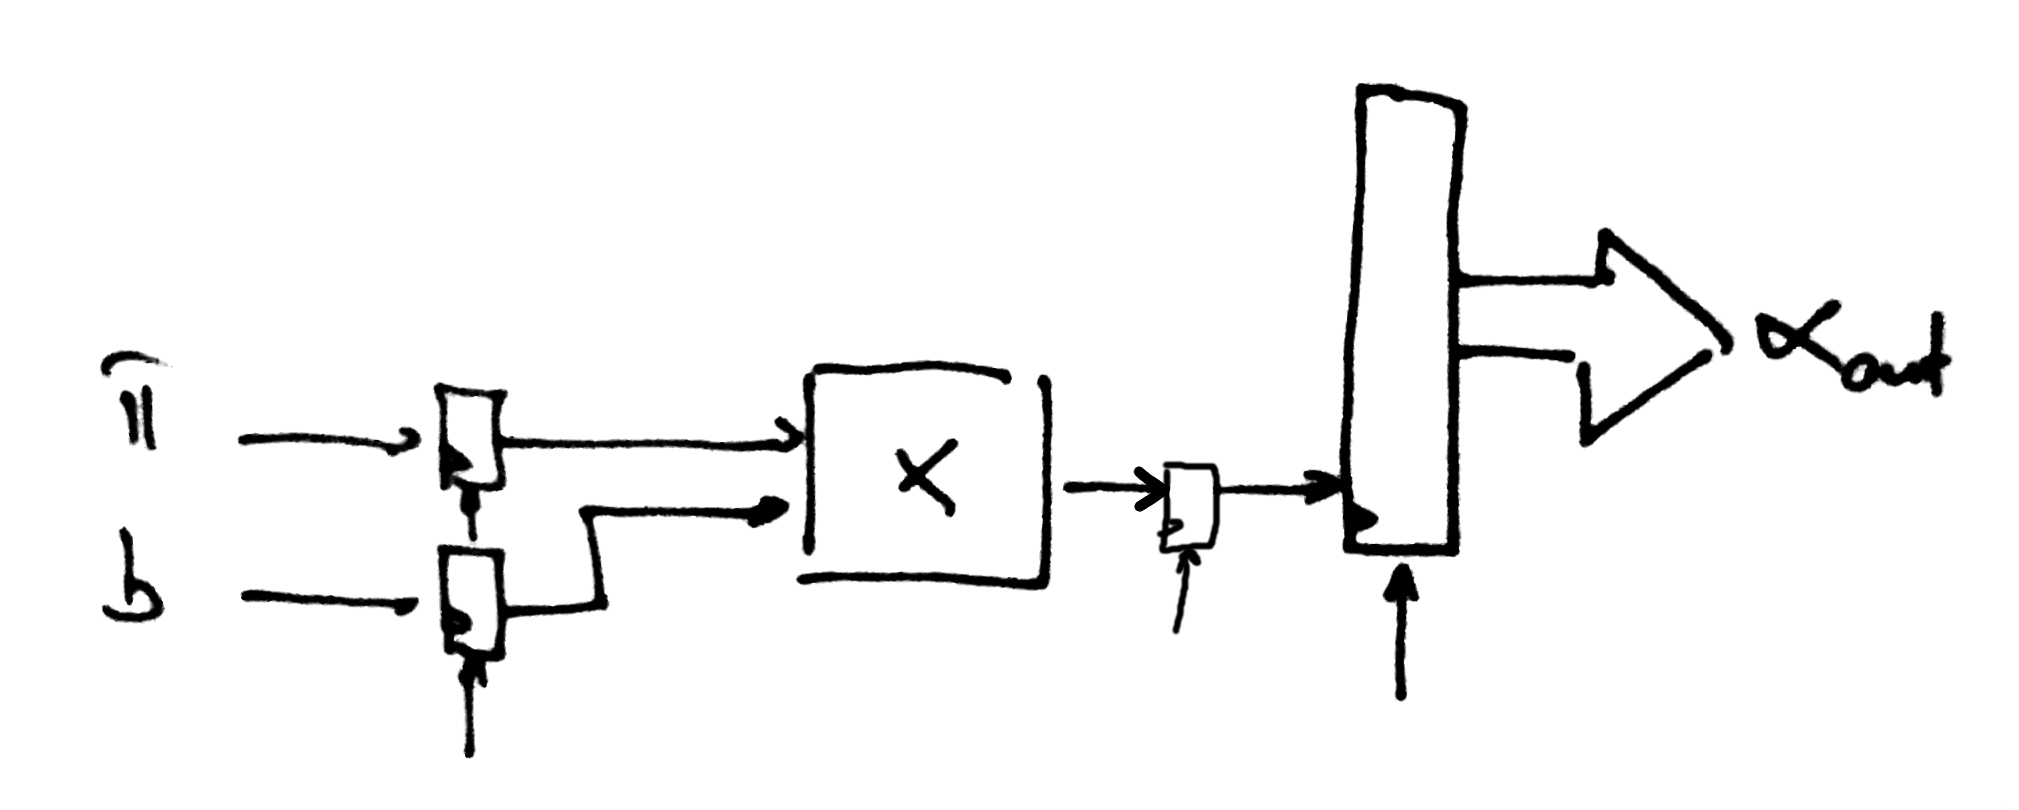
\includegraphics[width=1\columnwidth]{./schema/arch_init_s.png}
    \caption{initialisation step with one macc}
    \label{fig:init_s}
\end{figure}

%-------------------------------------------------------------------------------
%===============================================================================
\section{k-th forward variable}
\emph{\color{red}better title?}

\begin{itemize}
    \item one pipelined macc for the computation of all elements
    \item $ n $ pipelined macc, each computing one $ \alpha_k $
    \item use optimized matrix-vector-vector multiplication
        $ \alpha_{k+1} = tp * \alpha_k * b(o_k) $
        \cite{FCCM12_Kestur, ITNG07_Yang}
\end{itemize}

\begin{figure}
    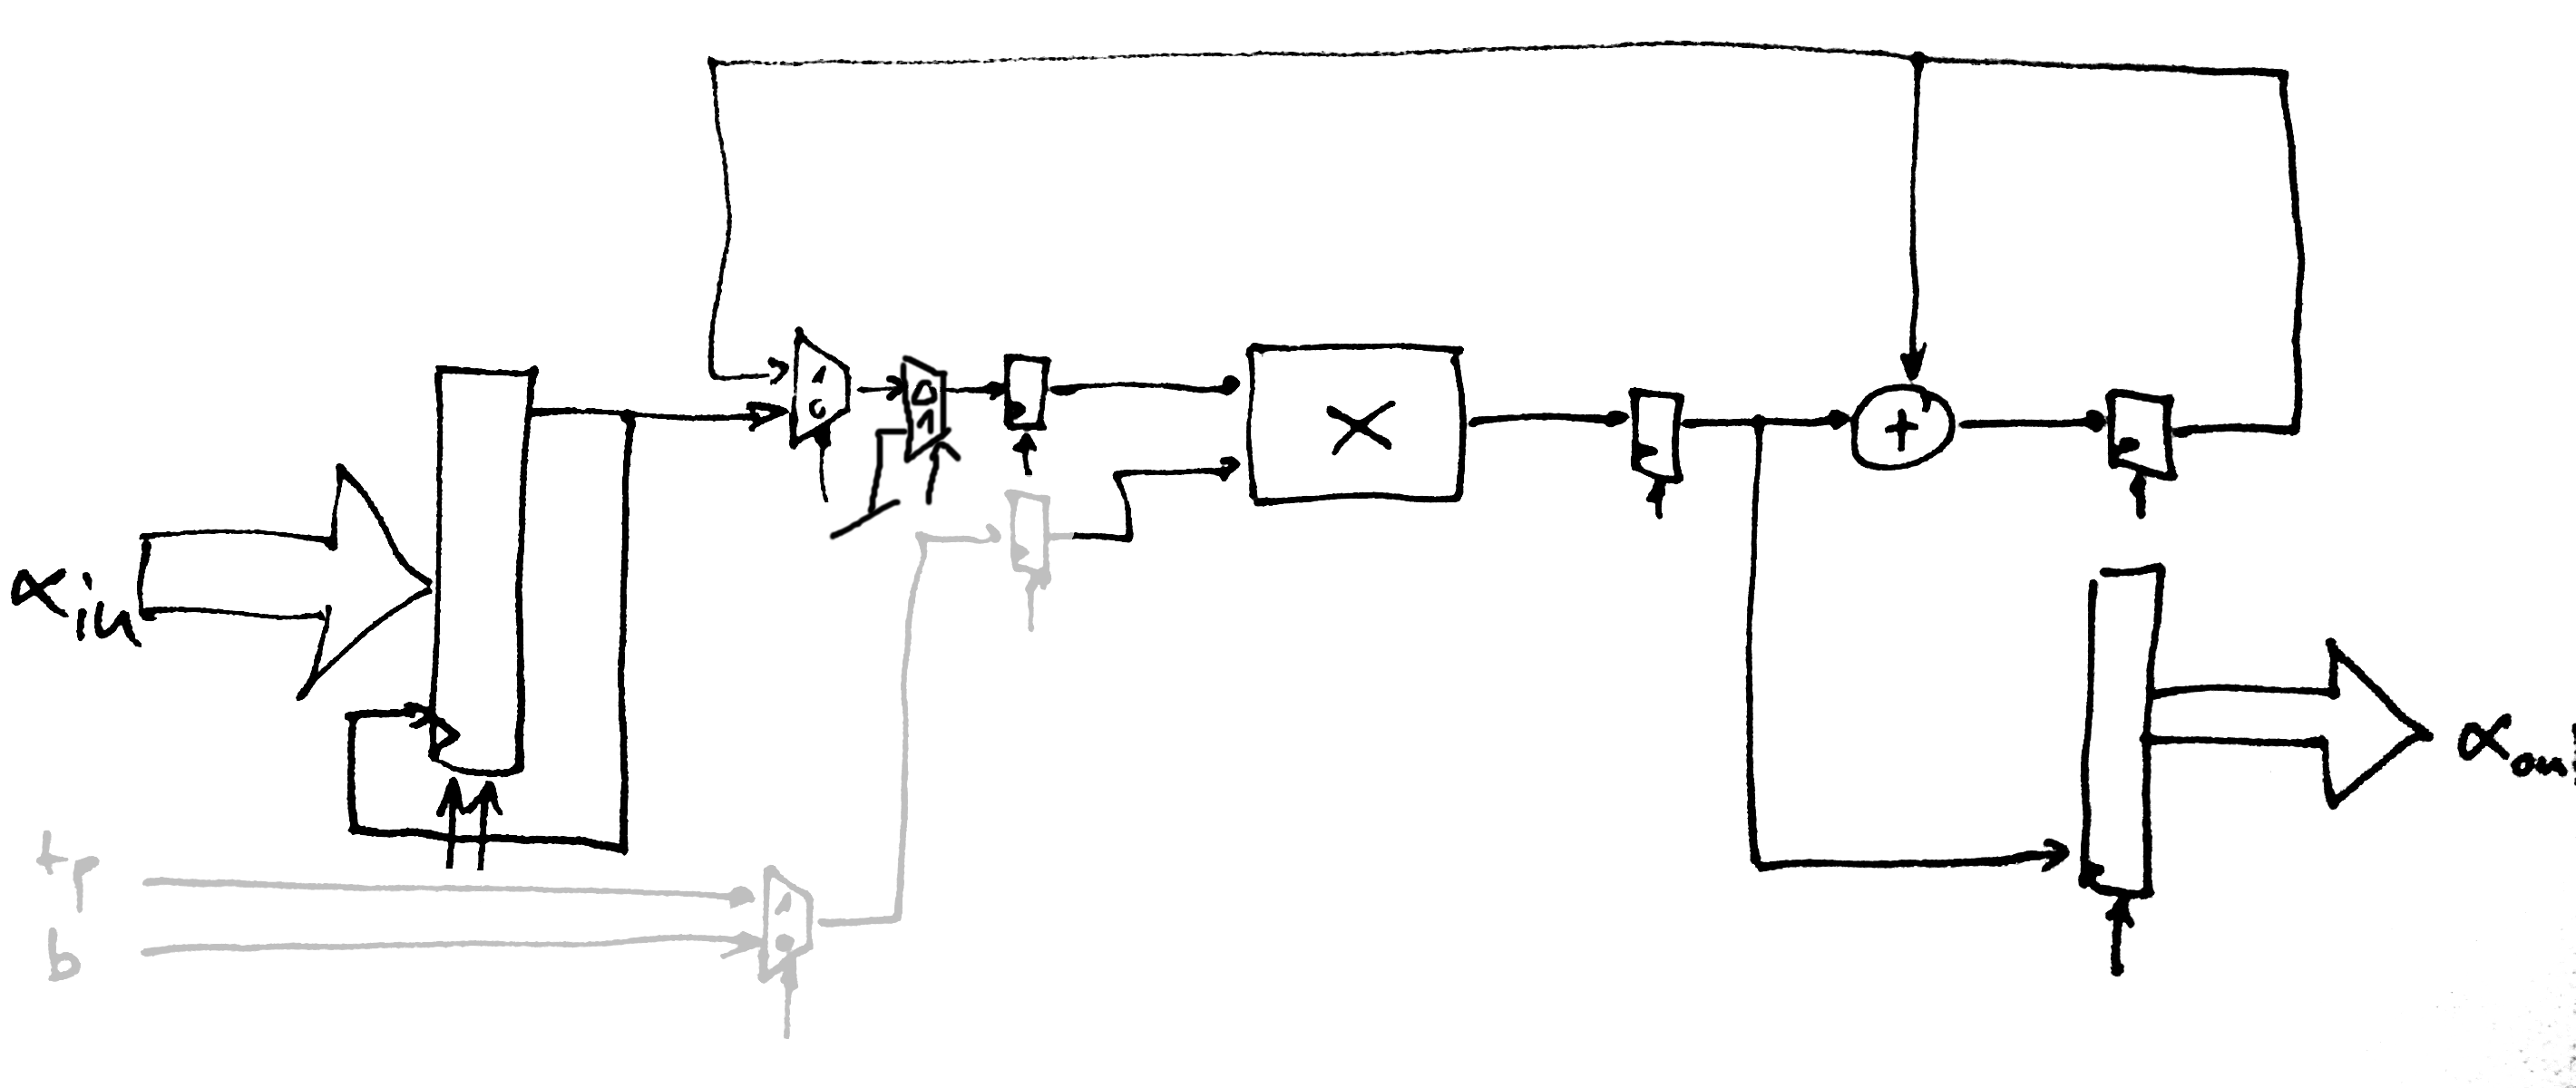
\includegraphics[width=1\columnwidth]{./schema/arch_step_s.png}
    \caption{k-th step with one macc unit}
    \label{fig:step_s}
\end{figure}
\begin{figure}
    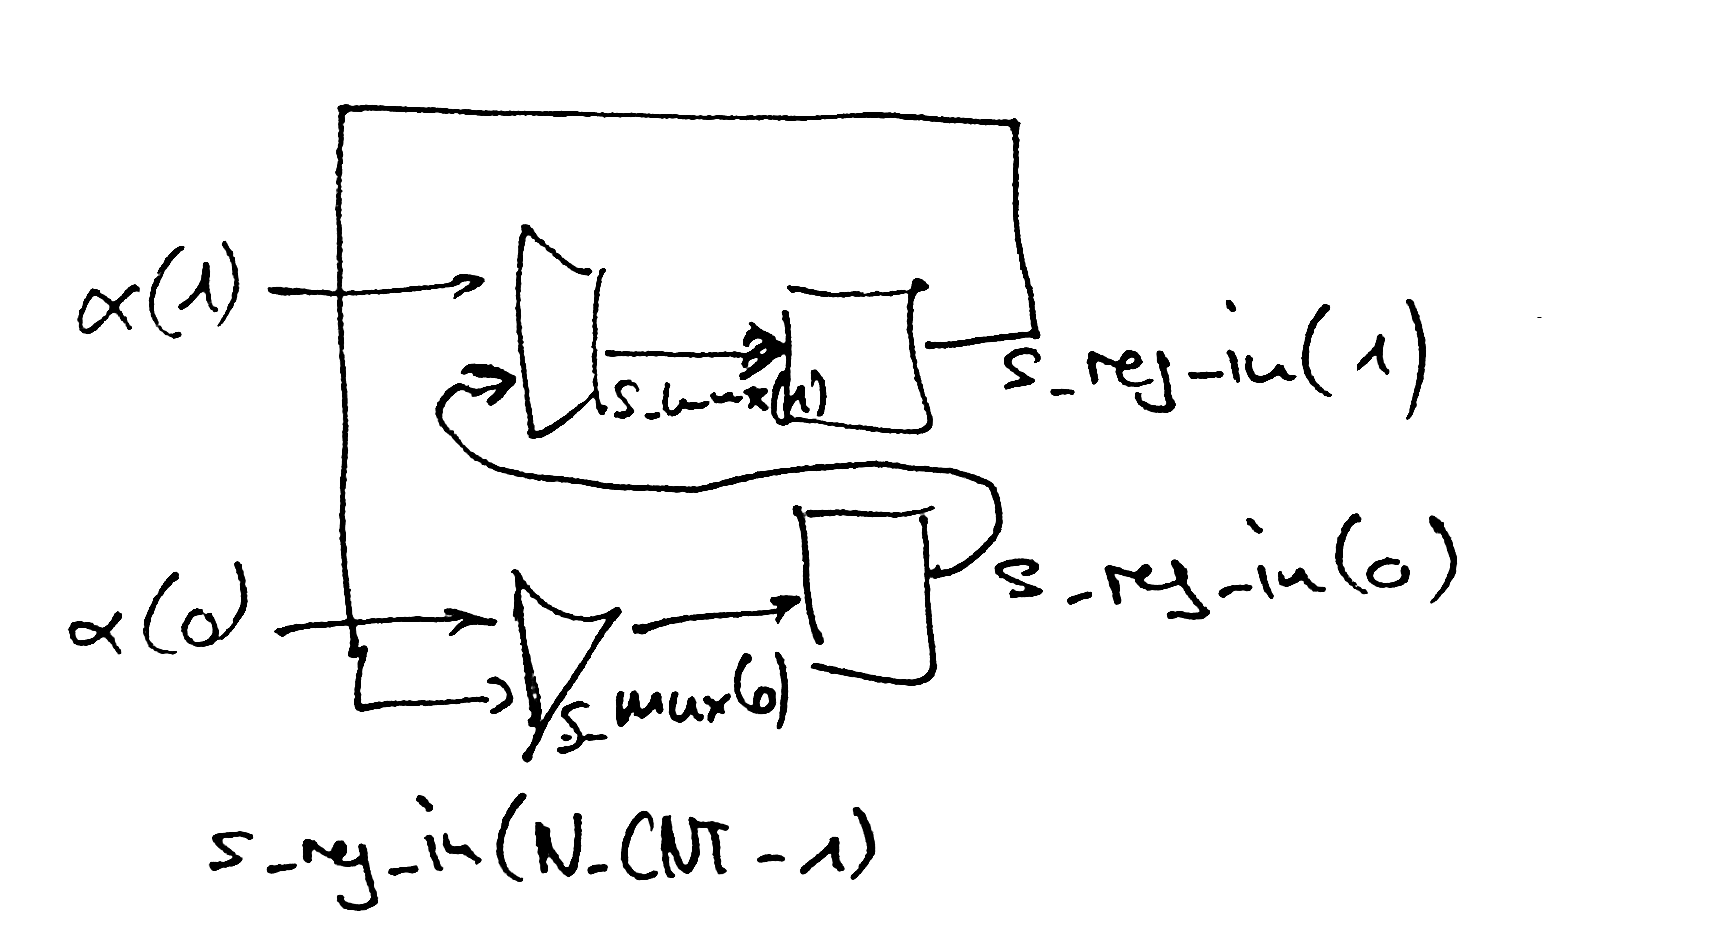
\includegraphics[width=1\columnwidth]{./schema/arch_shift_reg_s.png}
    \caption{example of input shift register with n=2}
    \label{fig:shift_reg_s}
\end{figure}

\begin{figure}
    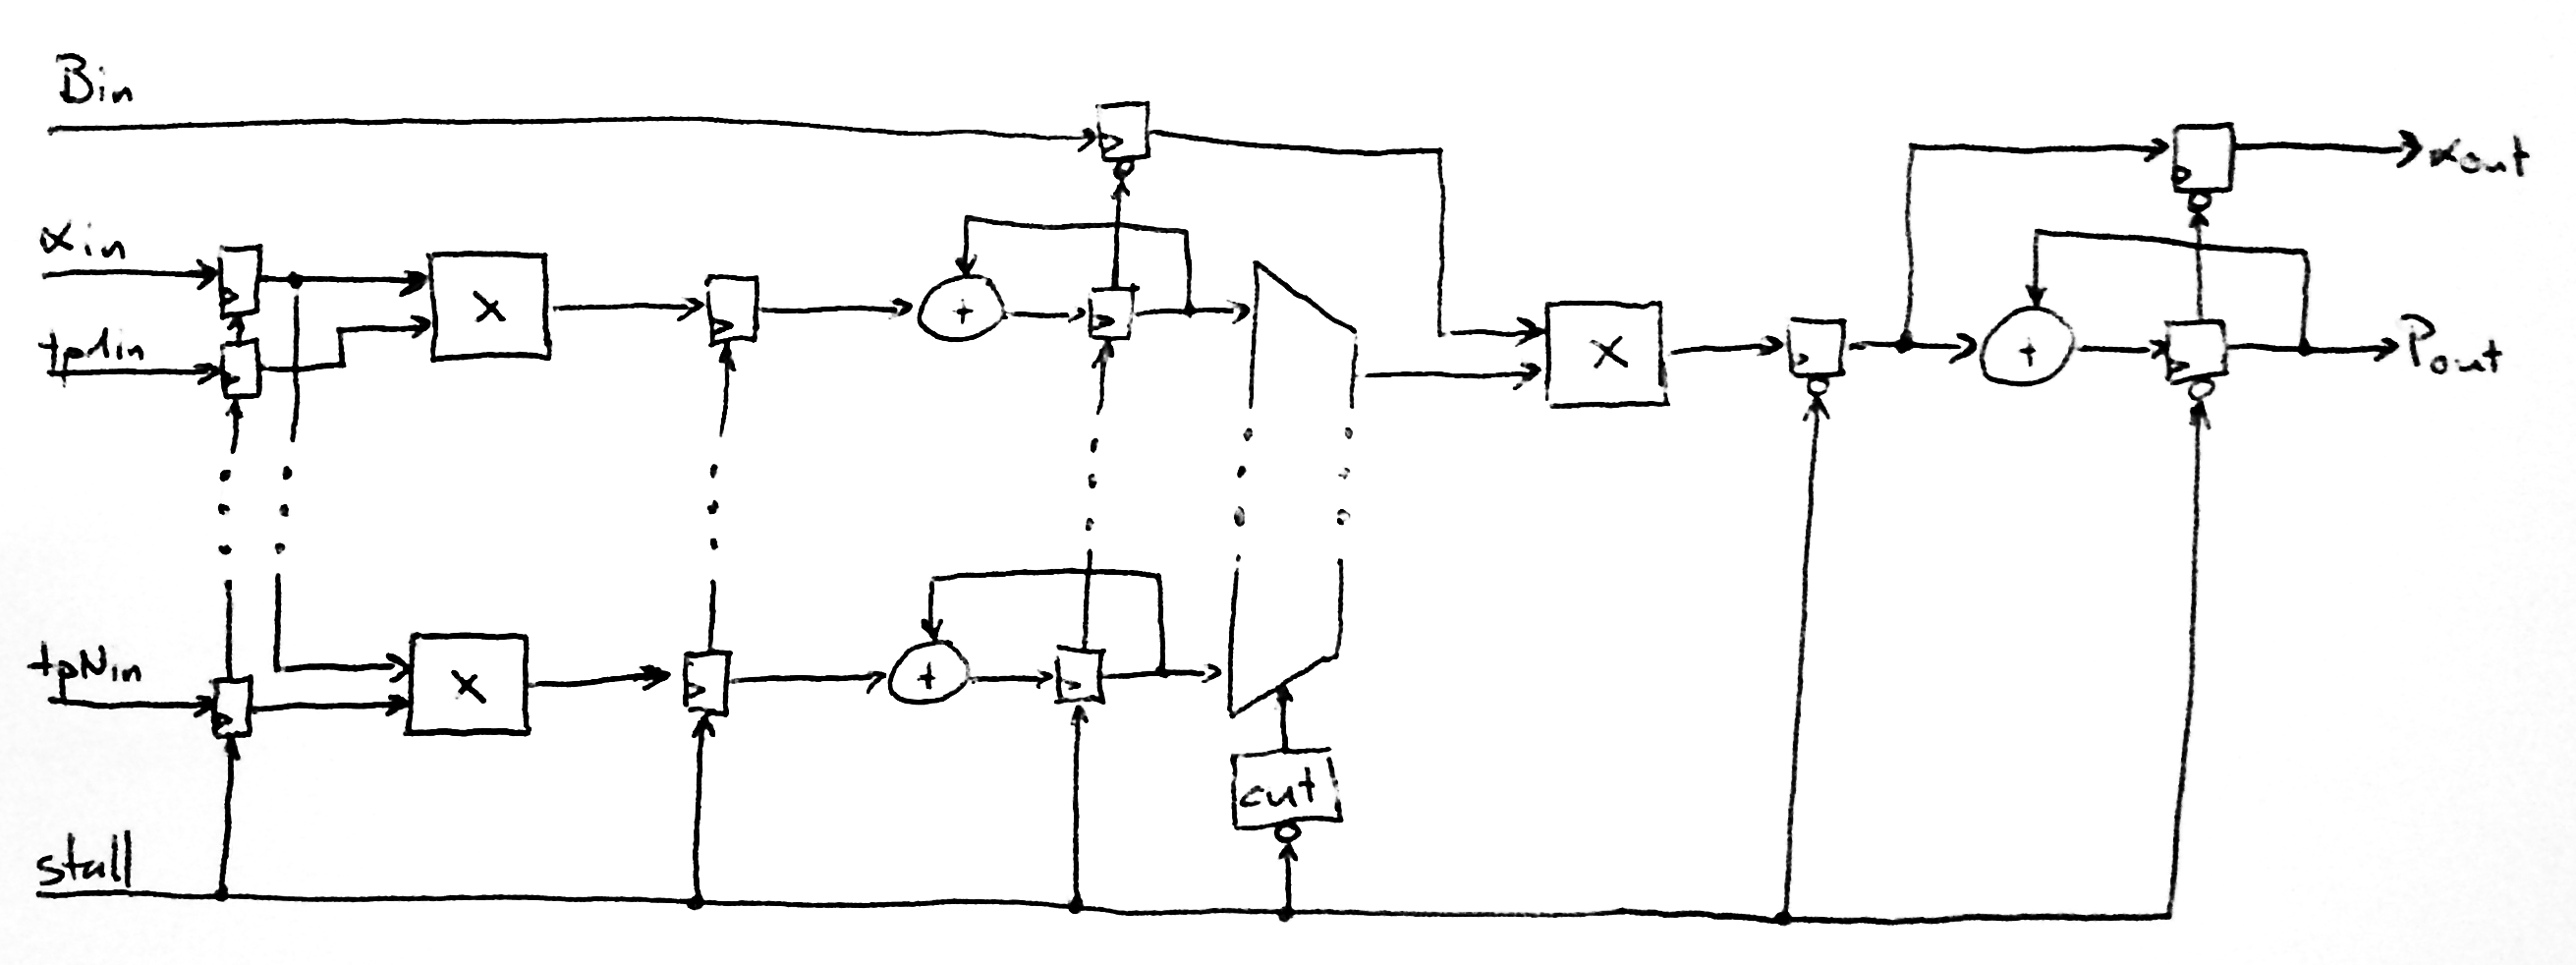
\includegraphics[width=1\columnwidth]{./schema/arch_step_p.png}
    \caption{k-th step with $ n+1 $ macc units and integrated computation of p
        (which is only needed at the last step)}
    \label{fig:step_p}
\end{figure}

\begin{figure}
    \centering
    % Generated with LaTeXDraw 2.0.8
% Wed Jun 25 15:35:51 CEST 2014
% \usepackage[usenames,dvipsnames]{pstricks}
% \usepackage{epsfig}
% \usepackage{pst-grad} % For gradients
% \usepackage{pst-plot} % For axes
\scalebox{1} % Change this value to rescale the drawing.
{
\begin{pspicture}(0,-2.62)(14.222813,2.62)
\pspolygon[linewidth=0.04](4.5809374,1.4)(4.9809375,1.2)(4.9809375,0.8)(4.5809374,0.6)
\pspolygon[linewidth=0.04](5.9809375,-2.2)(6.5809374,-2.0)(6.5809374,-1.2)(5.9809375,-1.0)
\pspolygon[linewidth=0.04](5.9809375,0.0)(6.7809377,0.2)(6.7809377,1.8)(5.9809375,2.0)
\psellipse[linewidth=0.04,dimen=outer](8.380938,1.0)(0.4,0.4)
\psline[linewidth=0.04cm](8.180938,0.8)(8.580937,1.2)
\psline[linewidth=0.04cm](8.180938,1.2)(8.580937,0.8)
\psline[linewidth=0.04cm](10.780937,1.2)(10.780937,0.8)
\psline[linewidth=0.04cm](10.580937,1.0)(10.980938,1.0)
\psellipse[linewidth=0.04,dimen=outer](10.780937,1.0)(0.4,0.4)
\psframe[linewidth=0.04,dimen=outer](11.980938,1.2)(11.580937,0.6)
\rput{-90.0}(10.950937,12.390938){\pstriangle[linewidth=0.016,dimen=outer](11.670938,0.64)(0.18,0.16)}
\psframe[linewidth=0.04,dimen=outer](9.980938,1.2)(9.580937,0.6)
\rput{-90.0}(8.950937,10.390938){\pstriangle[linewidth=0.016,dimen=outer](9.670938,0.64)(0.18,0.16)}
\psframe[linewidth=0.04,dimen=outer](7.5809374,1.2)(7.1809373,0.6)
\rput{-90.0}(6.5509377,7.9909377){\pstriangle[linewidth=0.016,dimen=outer](7.2709374,0.64)(0.18,0.16)}
\psframe[linewidth=0.04,dimen=outer](7.5809374,-1.4)(7.1809373,-2.0)
\rput{-90.0}(9.150937,5.3909373){\pstriangle[linewidth=0.016,dimen=outer](7.2709374,-1.96)(0.18,0.16)}
\psline[linewidth=0.04cm,arrowsize=0.05291667cm 2.0,arrowlength=1.4,arrowinset=0.4]{->}(7.5809374,1.0)(7.9809375,1.0)
\psline[linewidth=0.04cm,arrowsize=0.05291667cm 2.0,arrowlength=1.4,arrowinset=0.4]{->}(8.780937,1.0)(9.580937,1.0)
\psline[linewidth=0.04cm,arrowsize=0.05291667cm 2.0,arrowlength=1.4,arrowinset=0.4]{->}(9.980938,1.0)(10.380938,1.0)
\psline[linewidth=0.04cm,arrowsize=0.05291667cm 2.0,arrowlength=1.4,arrowinset=0.4]{->}(11.180938,1.0)(11.580937,1.0)
\psline[linewidth=0.04,arrowsize=0.05291667cm 2.0,arrowlength=1.4,arrowinset=0.4]{->}(11.980938,1.0)(12.380938,1.0)(12.380938,2.6)(10.780937,2.6)(10.780937,1.4)
\psline[linewidth=0.04cm,arrowsize=0.05291667cm 2.0,arrowlength=1.4,arrowinset=0.4]{->}(6.7809377,1.0)(7.1809373,1.0)
\psline[linewidth=0.04,arrowsize=0.05291667cm 2.0,arrowlength=1.4,arrowinset=0.4,dotsize=0.07055555cm 2.0]{*->}(10.780937,2.6)(5.3809376,2.6)(5.3809376,1.4)(5.9809375,1.4)
\psline[linewidth=0.04,arrowsize=0.05291667cm 2.0,arrowlength=1.4,arrowinset=0.4,dotsize=0.07055555cm 2.0]{*->}(9.180938,1.0)(9.180938,2.4)(5.5809374,2.4)(5.5809374,1.6)(5.9809375,1.6)
\psline[linewidth=0.04cm,arrowsize=0.05291667cm 2.0,arrowlength=1.4,arrowinset=0.4]{->}(6.5809374,-1.6)(7.1809373,-1.6)
\psline[linewidth=0.04,arrowsize=0.05291667cm 2.0,arrowlength=1.4,arrowinset=0.4]{->}(7.5809374,-1.6)(8.380938,-1.6)(8.380938,0.6)
\psline[linewidth=0.04,arrowsize=0.05291667cm 2.0,arrowlength=1.4,arrowinset=0.4,dotsize=0.07055555cm 2.0]{*->}(5.3809376,1.4)(5.3809376,1.2)(5.9809375,1.2)
\psline[linewidth=0.04,arrowsize=0.05291667cm 2.0,arrowlength=1.4,arrowinset=0.4]{->}(5.5809374,-0.2)(5.5809374,0.8)(5.9809375,0.8)
\psline[linewidth=0.04cm,dotsize=0.07055555cm 2.0,arrowsize=0.05291667cm 2.0,arrowlength=1.4,arrowinset=0.4]{*->}(5.5809374,0.6)(5.9809375,0.6)
\psline[linewidth=0.04cm,dotsize=0.07055555cm 2.0,arrowsize=0.05291667cm 2.0,arrowlength=1.4,arrowinset=0.4]{*->}(5.5809374,0.4)(5.9809375,0.4)
\psline[linewidth=0.04cm,dotsize=0.07055555cm 2.0,arrowsize=0.05291667cm 2.0,arrowlength=1.4,arrowinset=0.4]{*->}(5.5809374,0.2)(5.9809375,0.2)
\psline[linewidth=0.04cm](5.3809376,-0.4)(5.7809377,0.0)
\psline[linewidth=0.04cm,arrowsize=0.05291667cm 2.0,arrowlength=1.4,arrowinset=0.4]{->}(5.1809373,-1.4)(5.9809375,-1.4)
\psline[linewidth=0.04cm,arrowsize=0.05291667cm 2.0,arrowlength=1.4,arrowinset=0.4]{->}(5.1809373,-1.8)(5.9809375,-1.8)
\psline[linewidth=0.04cm,arrowsize=0.05291667cm 2.0,arrowlength=1.4,arrowinset=0.4]{->}(5.1809373,-2.0)(5.9809375,-2.0)
\psline[linewidth=0.04,arrowsize=0.05291667cm 2.0,arrowlength=1.4,arrowinset=0.4,dotsize=0.07055555cm 2.0]{*->}(5.5809374,-1.4)(5.5809374,-1.6)(5.9809375,-1.6)
\psline[linewidth=0.04,arrowsize=0.05291667cm 2.0,arrowlength=1.4,arrowinset=0.4,dotsize=0.07055555cm 2.0]{*->}(9.180938,1.0)(9.180938,0.0)(12.780937,0.0)
\psline[linewidth=0.04cm,arrowsize=0.05291667cm 2.0,arrowlength=1.4,arrowinset=0.4]{->}(4.9809375,1.0)(5.9809375,1.0)
\psline[linewidth=0.04cm,arrowsize=0.05291667cm 2.0,arrowlength=1.4,arrowinset=0.4]{->}(6.1809373,-0.4)(6.1809373,0.04)
\psline[linewidth=0.04cm,arrowsize=0.05291667cm 2.0,arrowlength=1.4,arrowinset=0.4]{->}(6.3809376,-0.4)(6.3809376,0.08)
\psline[linewidth=0.04cm,arrowsize=0.05291667cm 2.0,arrowlength=1.4,arrowinset=0.4]{->}(6.5809374,-0.4)(6.5809374,0.14)
\psline[linewidth=0.04cm,arrowsize=0.05291667cm 2.0,arrowlength=1.4,arrowinset=0.4]{->}(6.1809373,-2.6)(6.1809373,-2.14)
\psline[linewidth=0.04cm,arrowsize=0.05291667cm 2.0,arrowlength=1.4,arrowinset=0.4]{->}(6.3809376,-2.6)(6.3809376,-2.08)
\psline[linewidth=0.04cm,arrowsize=0.05291667cm 2.0,arrowlength=1.4,arrowinset=0.4]{->}(4.7809377,0.2)(4.7809377,0.68)
\psframe[linewidth=0.04,dimen=outer](4.1809373,1.0)(3.3809376,0.2)
\psframe[linewidth=0.04,dimen=outer](2.9809375,1.4)(2.1809375,0.6)
\psline[linewidth=0.04cm,arrowsize=0.05291667cm 2.0,arrowlength=1.4,arrowinset=0.4]{->}(4.1809373,0.8)(4.5809374,0.8)
\psline[linewidth=0.04cm,arrowsize=0.05291667cm 2.0,arrowlength=1.4,arrowinset=0.4]{->}(2.9809375,1.2)(4.5809374,1.2)
\psline[linewidth=0.04cm,arrowsize=0.05291667cm 2.0,arrowlength=1.4,arrowinset=0.4]{->}(1.3809375,0.4)(3.3809376,0.4)
\psline[linewidth=0.04,arrowsize=0.05291667cm 2.0,arrowlength=1.4,arrowinset=0.4,dotsize=0.07055555cm 2.0]{*->}(1.7809376,0.4)(1.7809376,0.8)(2.1809375,0.8)
\psline[linewidth=0.04cm,arrowsize=0.05291667cm 2.0,arrowlength=1.4,arrowinset=0.4]{->}(2.3809376,2.0)(2.3809376,1.4)
\psline[linewidth=0.04cm,arrowsize=0.05291667cm 2.0,arrowlength=1.4,arrowinset=0.4]{->}(2.5809374,2.0)(2.5809374,1.4)
\psline[linewidth=0.04cm,arrowsize=0.05291667cm 2.0,arrowlength=1.4,arrowinset=0.4]{->}(3.5809374,-0.4)(3.5809374,0.2)
\psline[linewidth=0.04cm,arrowsize=0.05291667cm 2.0,arrowlength=1.4,arrowinset=0.4]{->}(3.7809374,-0.4)(3.7809374,0.2)
\usefont{T1}{ptm}{m}{n}
\rput(13.072344,0.105){$\alpha_{out}$}
\usefont{T1}{ptm}{m}{n}
\rput(0.97234374,0.505){$\alpha_{in}$}
\usefont{T1}{ptm}{m}{n}
\rput(4.7723436,-1.295){$TP$}
\usefont{T1}{ptm}{m}{n}
\rput(4.6923437,-1.695){$B(O_k)$}
\usefont{T1}{ptm}{m}{n}
\rput(4.6223435,-2.095){$F_{shift}$}
\usefont{T1}{ptm}{m}{n}
\rput(2.5801563,1.005){\scriptsize MEM}
\usefont{T1}{ptm}{m}{n}
\rput(3.7801561,0.605){\scriptsize MEM}
\end{pspicture} 
}


    \caption{Implementation of one step in a pipelined architecture, including
        scaling}
    \label{fig:step_s}
\end{figure}

%-------------------------------------------------------------------------------
%===============================================================================
\section{Scaling}

\begin{figure}
    \centering
    % Generated with LaTeXDraw 2.0.8
% Wed Jun 25 14:45:20 CEST 2014
% \usepackage[usenames,dvipsnames]{pstricks}
% \usepackage{epsfig}
% \usepackage{pst-grad} % For gradients
% \usepackage{pst-plot} % For axes
\scalebox{1} % Change this value to rescale the drawing.
{
\begin{pspicture}(0,-4.6292186)(12.402813,4.6692185)
\psellipse[linewidth=0.04,dimen=outer](6.5809374,1.5707812)(0.4,0.4)
\psellipse[linewidth=0.04,dimen=outer](4.9809375,1.5707812)(0.4,0.4)
\psellipse[linewidth=0.04,dimen=outer](3.3809376,1.5707812)(0.4,0.4)
\psellipse[linewidth=0.04,dimen=outer](1.7809376,1.5707812)(0.4,0.4)
\psline[linewidth=0.04cm](1.5809375,1.7707813)(1.9809375,1.3707813)
\psline[linewidth=0.04cm](1.5809375,1.3707813)(1.9809375,1.7707813)
\psline[linewidth=0.04cm](3.3809376,1.7707813)(3.3809376,1.3707813)
\psline[linewidth=0.04cm](3.1809375,1.5707812)(3.5809374,1.5707812)
\psline[linewidth=0.04cm](6.3809376,1.7707813)(6.7809377,1.3707813)
\psline[linewidth=0.04cm](6.3809376,1.3707813)(6.7809377,1.7707813)
\psline[linewidth=0.04cm,arrowsize=0.05291667cm 2.0,arrowlength=1.4,arrowinset=0.4]{->}(2.1809375,1.5707812)(2.9809375,1.5707812)
\psline[linewidth=0.04cm,arrowsize=0.05291667cm 2.0,arrowlength=1.4,arrowinset=0.4]{->}(3.7809374,1.5707812)(4.5809374,1.5707812)
\psline[linewidth=0.04cm,arrowsize=0.05291667cm 2.0,arrowlength=1.4,arrowinset=0.4]{->}(5.3809376,1.5707812)(6.1809373,1.5707812)
\psline[linewidth=0.04cm,arrowsize=0.05291667cm 2.0,arrowlength=1.4,arrowinset=0.4]{->}(6.9809375,1.5707812)(7.7809377,1.5707812)
\psline[linewidth=0.04cm,arrowsize=0.05291667cm 2.0,arrowlength=1.4,arrowinset=0.4]{->}(6.5809374,2.3707812)(6.5809374,1.9707812)
\psline[linewidth=0.04cm,arrowsize=0.05291667cm 2.0,arrowlength=1.4,arrowinset=0.4]{->}(0.5809375,1.5707812)(1.3809375,1.5707812)
\psellipse[linewidth=0.04,dimen=outer](6.5809374,-0.22921875)(0.4,0.4)
\psellipse[linewidth=0.04,dimen=outer](4.9809375,-0.22921875)(0.4,0.4)
\psellipse[linewidth=0.04,dimen=outer](3.3809376,-0.22921875)(0.4,0.4)
\psellipse[linewidth=0.04,dimen=outer](1.7809376,-0.22921875)(0.4,0.4)
\psline[linewidth=0.04cm](1.5809375,-0.02921875)(1.9809375,-0.42921874)
\psline[linewidth=0.04cm](1.5809375,-0.42921874)(1.9809375,-0.02921875)
\psline[linewidth=0.04cm](3.3809376,-0.02921875)(3.3809376,-0.42921874)
\psline[linewidth=0.04cm](3.1809375,-0.22921875)(3.5809374,-0.22921875)
\psline[linewidth=0.04cm](6.3809376,-0.02921875)(6.7809377,-0.42921874)
\psline[linewidth=0.04cm](6.3809376,-0.42921874)(6.7809377,-0.02921875)
\psline[linewidth=0.04cm,arrowsize=0.05291667cm 2.0,arrowlength=1.4,arrowinset=0.4]{->}(2.1809375,-0.22921875)(2.9809375,-0.22921875)
\psline[linewidth=0.04cm,arrowsize=0.05291667cm 2.0,arrowlength=1.4,arrowinset=0.4]{->}(3.7809374,-0.22921875)(4.5809374,-0.22921875)
\psline[linewidth=0.04cm,arrowsize=0.05291667cm 2.0,arrowlength=1.4,arrowinset=0.4]{->}(5.3809376,-0.22921875)(6.1809373,-0.22921875)
\psline[linewidth=0.04cm,arrowsize=0.05291667cm 2.0,arrowlength=1.4,arrowinset=0.4]{->}(6.9809375,-0.22921875)(7.7809377,-0.22921875)
\psline[linewidth=0.04cm,arrowsize=0.05291667cm 2.0,arrowlength=1.4,arrowinset=0.4]{->}(6.5809374,0.57078123)(6.5809374,0.17078125)
\psline[linewidth=0.04,arrowsize=0.05291667cm 2.0,arrowlength=1.4,arrowinset=0.4,dotsize=0.07055555cm 2.0]{*->}(7.3809376,1.5707812)(7.3809376,0.97078127)(1.7809376,0.97078127)(1.7809376,0.17078125)
\psline[linewidth=0.04,arrowsize=0.05291667cm 2.0,arrowlength=1.4,arrowinset=0.4,dotsize=0.07055555cm 2.0]{*->}(4.1809373,-0.22921875)(4.1809373,0.57078123)(3.3809376,0.57078123)(3.3809376,0.17078125)
\psline[linewidth=0.04,arrowsize=0.05291667cm 2.0,arrowlength=1.4,arrowinset=0.4]{->}(8.580937,1.5707812)(8.980938,1.5707812)(8.980938,0.7707813)(4.9809375,0.7707813)(4.9809375,0.17078125)
\psellipse[linewidth=0.04,dimen=outer](6.5809374,3.3707812)(0.4,0.4)
\psline[linewidth=0.04cm](6.3809376,3.5707812)(6.7809377,3.1707811)
\psline[linewidth=0.04cm](6.3809376,3.1707811)(6.7809377,3.5707812)
\psline[linewidth=0.04,arrowsize=0.05291667cm 2.0,arrowlength=1.4,arrowinset=0.4,dotsize=0.07055555cm 2.0]{*->}(7.3809376,3.3707812)(7.3809376,2.7707813)(1.7809376,2.7707813)(1.7809376,1.9707812)
\psellipse[linewidth=0.04,dimen=outer](8.180938,3.3707812)(0.4,0.4)
\psline[linewidth=0.04cm,arrowsize=0.05291667cm 2.0,arrowlength=1.4,arrowinset=0.4]{->}(6.9809375,3.3707812)(7.7809377,3.3707812)
\psline[linewidth=0.04,arrowsize=0.05291667cm 2.0,arrowlength=1.4,arrowinset=0.4]{->}(8.580937,3.3707812)(8.980938,3.3707812)(8.980938,2.5707812)(4.9809375,2.5707812)(4.9809375,1.9707812)
\psline[linewidth=0.04cm,arrowsize=0.05291667cm 2.0,arrowlength=1.4,arrowinset=0.4]{->}(5.5809374,3.3707812)(6.1809373,3.3707812)
\psline[linewidth=0.04cm,arrowsize=0.05291667cm 2.0,arrowlength=1.4,arrowinset=0.4]{->}(6.5809374,4.170781)(6.5809374,3.7707813)
\psline[linewidth=0.04cm,dotsize=0.07055555cm 2.0]{*-}(7.3809376,-0.22921875)(7.3809376,-0.82921875)
\psline[linewidth=0.04cm,linestyle=dotted,dotsep=0.16cm](7.3809376,-0.82921875)(7.3809376,-1.4292188)
\psellipse[linewidth=0.04,dimen=outer](6.5809374,-2.8292189)(0.4,0.4)
\psellipse[linewidth=0.04,dimen=outer](4.9809375,-2.8292189)(0.4,0.4)
\psellipse[linewidth=0.04,dimen=outer](3.3809376,-2.8292189)(0.4,0.4)
\psellipse[linewidth=0.04,dimen=outer](1.7809376,-2.8292189)(0.4,0.4)
\psline[linewidth=0.04cm](1.5809375,-2.6292188)(1.9809375,-3.0292187)
\psline[linewidth=0.04cm](1.5809375,-3.0292187)(1.9809375,-2.6292188)
\psline[linewidth=0.04cm](3.3809376,-2.6292188)(3.3809376,-3.0292187)
\psline[linewidth=0.04cm](3.1809375,-2.8292189)(3.5809374,-2.8292189)
\psline[linewidth=0.04cm](6.3809376,-2.6292188)(6.7809377,-3.0292187)
\psline[linewidth=0.04cm](6.3809376,-3.0292187)(6.7809377,-2.6292188)
\psline[linewidth=0.04cm,arrowsize=0.05291667cm 2.0,arrowlength=1.4,arrowinset=0.4]{->}(2.1809375,-2.8292189)(2.9809375,-2.8292189)
\psline[linewidth=0.04cm,arrowsize=0.05291667cm 2.0,arrowlength=1.4,arrowinset=0.4]{->}(3.7809374,-2.8292189)(4.5809374,-2.8292189)
\psline[linewidth=0.04cm,arrowsize=0.05291667cm 2.0,arrowlength=1.4,arrowinset=0.4]{->}(5.3809376,-2.8292189)(6.1809373,-2.8292189)
\psline[linewidth=0.04cm,arrowsize=0.05291667cm 2.0,arrowlength=1.4,arrowinset=0.4]{->}(6.9809375,-2.8292189)(7.7809377,-2.8292189)
\psline[linewidth=0.04cm,arrowsize=0.05291667cm 2.0,arrowlength=1.4,arrowinset=0.4]{->}(6.5809374,-2.0292187)(6.5809374,-2.4292188)
\psline[linewidth=0.04,arrowsize=0.05291667cm 2.0,arrowlength=1.4,arrowinset=0.4]{->}(7.3809376,-1.4292188)(7.3809376,-1.6292187)(1.7809376,-1.6292187)(1.7809376,-2.4292188)
\psline[linewidth=0.04,arrowsize=0.05291667cm 2.0,arrowlength=1.4,arrowinset=0.4,dotsize=0.07055555cm 2.0]{*->}(4.1809373,-2.8292189)(4.1809373,-2.0292187)(3.3809376,-2.0292187)(3.3809376,-2.4292188)
\psline[linewidth=0.04](8.580937,-0.22921875)(8.980938,-0.22921875)(8.980938,-0.82921875)
\psline[linewidth=0.04cm,linestyle=dotted,dotsep=0.16cm](8.980938,-0.82921875)(8.980938,-1.4292188)
\psline[linewidth=0.04,arrowsize=0.05291667cm 2.0,arrowlength=1.4,arrowinset=0.4]{->}(8.980938,-1.4292188)(8.980938,-1.8292187)(4.9809375,-1.8292187)(4.9809375,-2.4292188)
\psellipse[linewidth=0.04,dimen=outer](9.980938,1.5707812)(0.4,0.4)
\psline[linewidth=0.04cm](9.980938,1.7707813)(9.980938,1.3707813)
\psline[linewidth=0.04cm](9.780937,1.5707812)(10.180938,1.5707812)
\psellipse[linewidth=0.04,dimen=outer](9.980938,-0.22921875)(0.4,0.4)
\psline[linewidth=0.04cm](9.980938,-0.02921875)(9.980938,-0.42921874)
\psline[linewidth=0.04cm](9.780937,-0.22921875)(10.180938,-0.22921875)
\psellipse[linewidth=0.04,dimen=outer](9.980938,-2.8292189)(0.4,0.4)
\psline[linewidth=0.04cm](9.980938,-2.6292188)(9.980938,-3.0292187)
\psline[linewidth=0.04cm](9.780937,-2.8292189)(10.180938,-2.8292189)
\psline[linewidth=0.04cm,dotsize=0.07055555cm 2.0,arrowsize=0.05291667cm 2.0,arrowlength=1.4,arrowinset=0.4]{*->}(8.980938,1.5707812)(9.580937,1.5707812)
\psline[linewidth=0.04cm,dotsize=0.07055555cm 2.0,arrowsize=0.05291667cm 2.0,arrowlength=1.4,arrowinset=0.4]{*->}(8.980938,-0.22921875)(9.580937,-0.22921875)
\psline[linewidth=0.04cm,arrowsize=0.05291667cm 2.0,arrowlength=1.4,arrowinset=0.4]{->}(8.580937,-2.8292189)(9.580937,-2.8292189)
\psline[linewidth=0.04,arrowsize=0.05291667cm 2.0,arrowlength=1.4,arrowinset=0.4,dotsize=0.07055555cm 2.0]{*->}(8.980938,3.3707812)(9.980938,3.3707812)(9.980938,1.9707812)
\psline[linewidth=0.04cm,arrowsize=0.05291667cm 2.0,arrowlength=1.4,arrowinset=0.4]{->}(9.980938,1.1707813)(9.980938,0.17078125)
\psline[linewidth=0.04cm,arrowsize=0.05291667cm 2.0,arrowlength=1.4,arrowinset=0.4]{->}(9.980938,-1.4292188)(9.980938,-2.4292188)
\psline[linewidth=0.04cm](9.980938,-0.62921876)(9.980938,-0.82921875)
\psline[linewidth=0.04cm,linestyle=dotted,dotsep=0.16cm](9.980938,-0.82921875)(9.980938,-1.4292188)
\psline[linewidth=0.04cm,arrowsize=0.05291667cm 2.0,arrowlength=1.4,arrowinset=0.4]{->}(10.380938,-2.8292189)(10.980938,-2.8292189)
\psellipse[linewidth=0.04,dimen=outer](8.180938,-4.229219)(0.4,0.4)
\psline[linewidth=0.04cm](8.180938,-4.0292187)(8.180938,-4.429219)
\psline[linewidth=0.04cm](7.9809375,-4.229219)(8.380938,-4.229219)
\psline[linewidth=0.04,arrowsize=0.05291667cm 2.0,arrowlength=1.4,arrowinset=0.4,dotsize=0.07055555cm 2.0]{*->}(7.3809376,-2.8292189)(7.3809376,-4.229219)(7.7809377,-4.229219)
\psline[linewidth=0.04cm,arrowsize=0.05291667cm 2.0,arrowlength=1.4,arrowinset=0.4]{->}(8.580937,-4.229219)(10.980938,-4.229219)
\psline[linewidth=0.04,arrowsize=0.05291667cm 2.0,arrowlength=1.4,arrowinset=0.4,dotsize=0.07055555cm 2.0]{*->}(8.980938,-4.229219)(8.980938,-3.4292188)(8.180938,-3.4292188)(8.180938,-3.8292189)
\usefont{T1}{ptm}{m}{n}
\rput(8.178906,3.3707812){\footnotesize LZC}
\psellipse[linewidth=0.04,dimen=outer](8.180938,1.5707812)(0.4,0.4)
\usefont{T1}{ptm}{m}{n}
\rput(8.178906,1.5707812){\footnotesize LZC}
\psellipse[linewidth=0.04,dimen=outer](8.180938,-0.22921875)(0.4,0.4)
\usefont{T1}{ptm}{m}{n}
\rput(8.178906,-0.22921875){\footnotesize LZC}
\psellipse[linewidth=0.04,dimen=outer](8.180938,-2.8292189)(0.4,0.4)
\usefont{T1}{ptm}{m}{n}
\rput(8.178906,-2.8292189){\footnotesize LZC}
\usefont{T1}{ptm}{m}{n}
\rput(6.6923437,4.4757814){$B(O_k)$}
\usefont{T1}{ptm}{m}{n}
\rput(5.322344,3.4757812){$\pi$}
\usefont{T1}{ptm}{m}{n}
\rput(0.37234375,1.6757812){$TP$}
\psline[linewidth=0.04,arrowsize=0.05291667cm 2.0,arrowlength=1.4,arrowinset=0.4,dotsize=0.07055555cm 2.0]{*->}(0.9809375,1.5707812)(0.9809375,-0.22921875)(1.3809375,-0.22921875)
\usefont{T1}{ptm}{m}{n}
\rput(11.212344,-2.7242188){$P_s$}
\usefont{T1}{ptm}{m}{n}
\rput(11.462344,-4.124219){$F_{scale}$}
\psline[linewidth=0.04](5.1809373,1.7707813)(4.9809375,1.5707812)(5.1809373,1.3707813)
\psline[linewidth=0.04](4.9809375,-0.02921875)(4.7809377,-0.22921875)(4.9809375,-0.42921874)
\psline[linewidth=0.04](5.1809373,-0.02921875)(4.9809375,-0.22921875)(5.1809373,-0.42921874)
\psline[linewidth=0.04](4.9809375,-2.6292188)(4.7809377,-2.8292189)(4.9809375,-3.0292187)
\psline[linewidth=0.04](5.1809373,-2.6292188)(4.9809375,-2.8292189)(5.1809373,-3.0292187)
\psline[linewidth=0.04](4.9809375,1.7707813)(4.7809377,1.5707812)(4.9809375,1.3707813)
\psline[linewidth=0.04cm,dotsize=0.07055555cm 2.0]{*-}(0.9809375,-0.22921875)(0.9809375,-0.82921875)
\psline[linewidth=0.04cm,linestyle=dotted,dotsep=0.16cm](0.9809375,-0.82921875)(0.9809375,-1.4292188)
\psline[linewidth=0.04,arrowsize=0.05291667cm 2.0,arrowlength=1.4,arrowinset=0.4]{->}(0.9809375,-1.4292188)(0.9809375,-2.8292189)(1.3809375,-2.8292189)
\psline[linewidth=0.04,arrowsize=0.05291667cm 2.0,arrowlength=1.4,arrowinset=0.4,dotsize=0.07055555cm 2.0]{*->}(4.1809373,1.5707812)(4.1809373,2.3707812)(3.3809376,2.3707812)(3.3809376,1.9707812)
\end{pspicture} 
}


    \caption{Simple scaling with shifter}
    \label{fig:scale}
\end{figure}

%-------------------------------------------------------------------------------
%===============================================================================
\section{serial controller}

\begin{figure}
    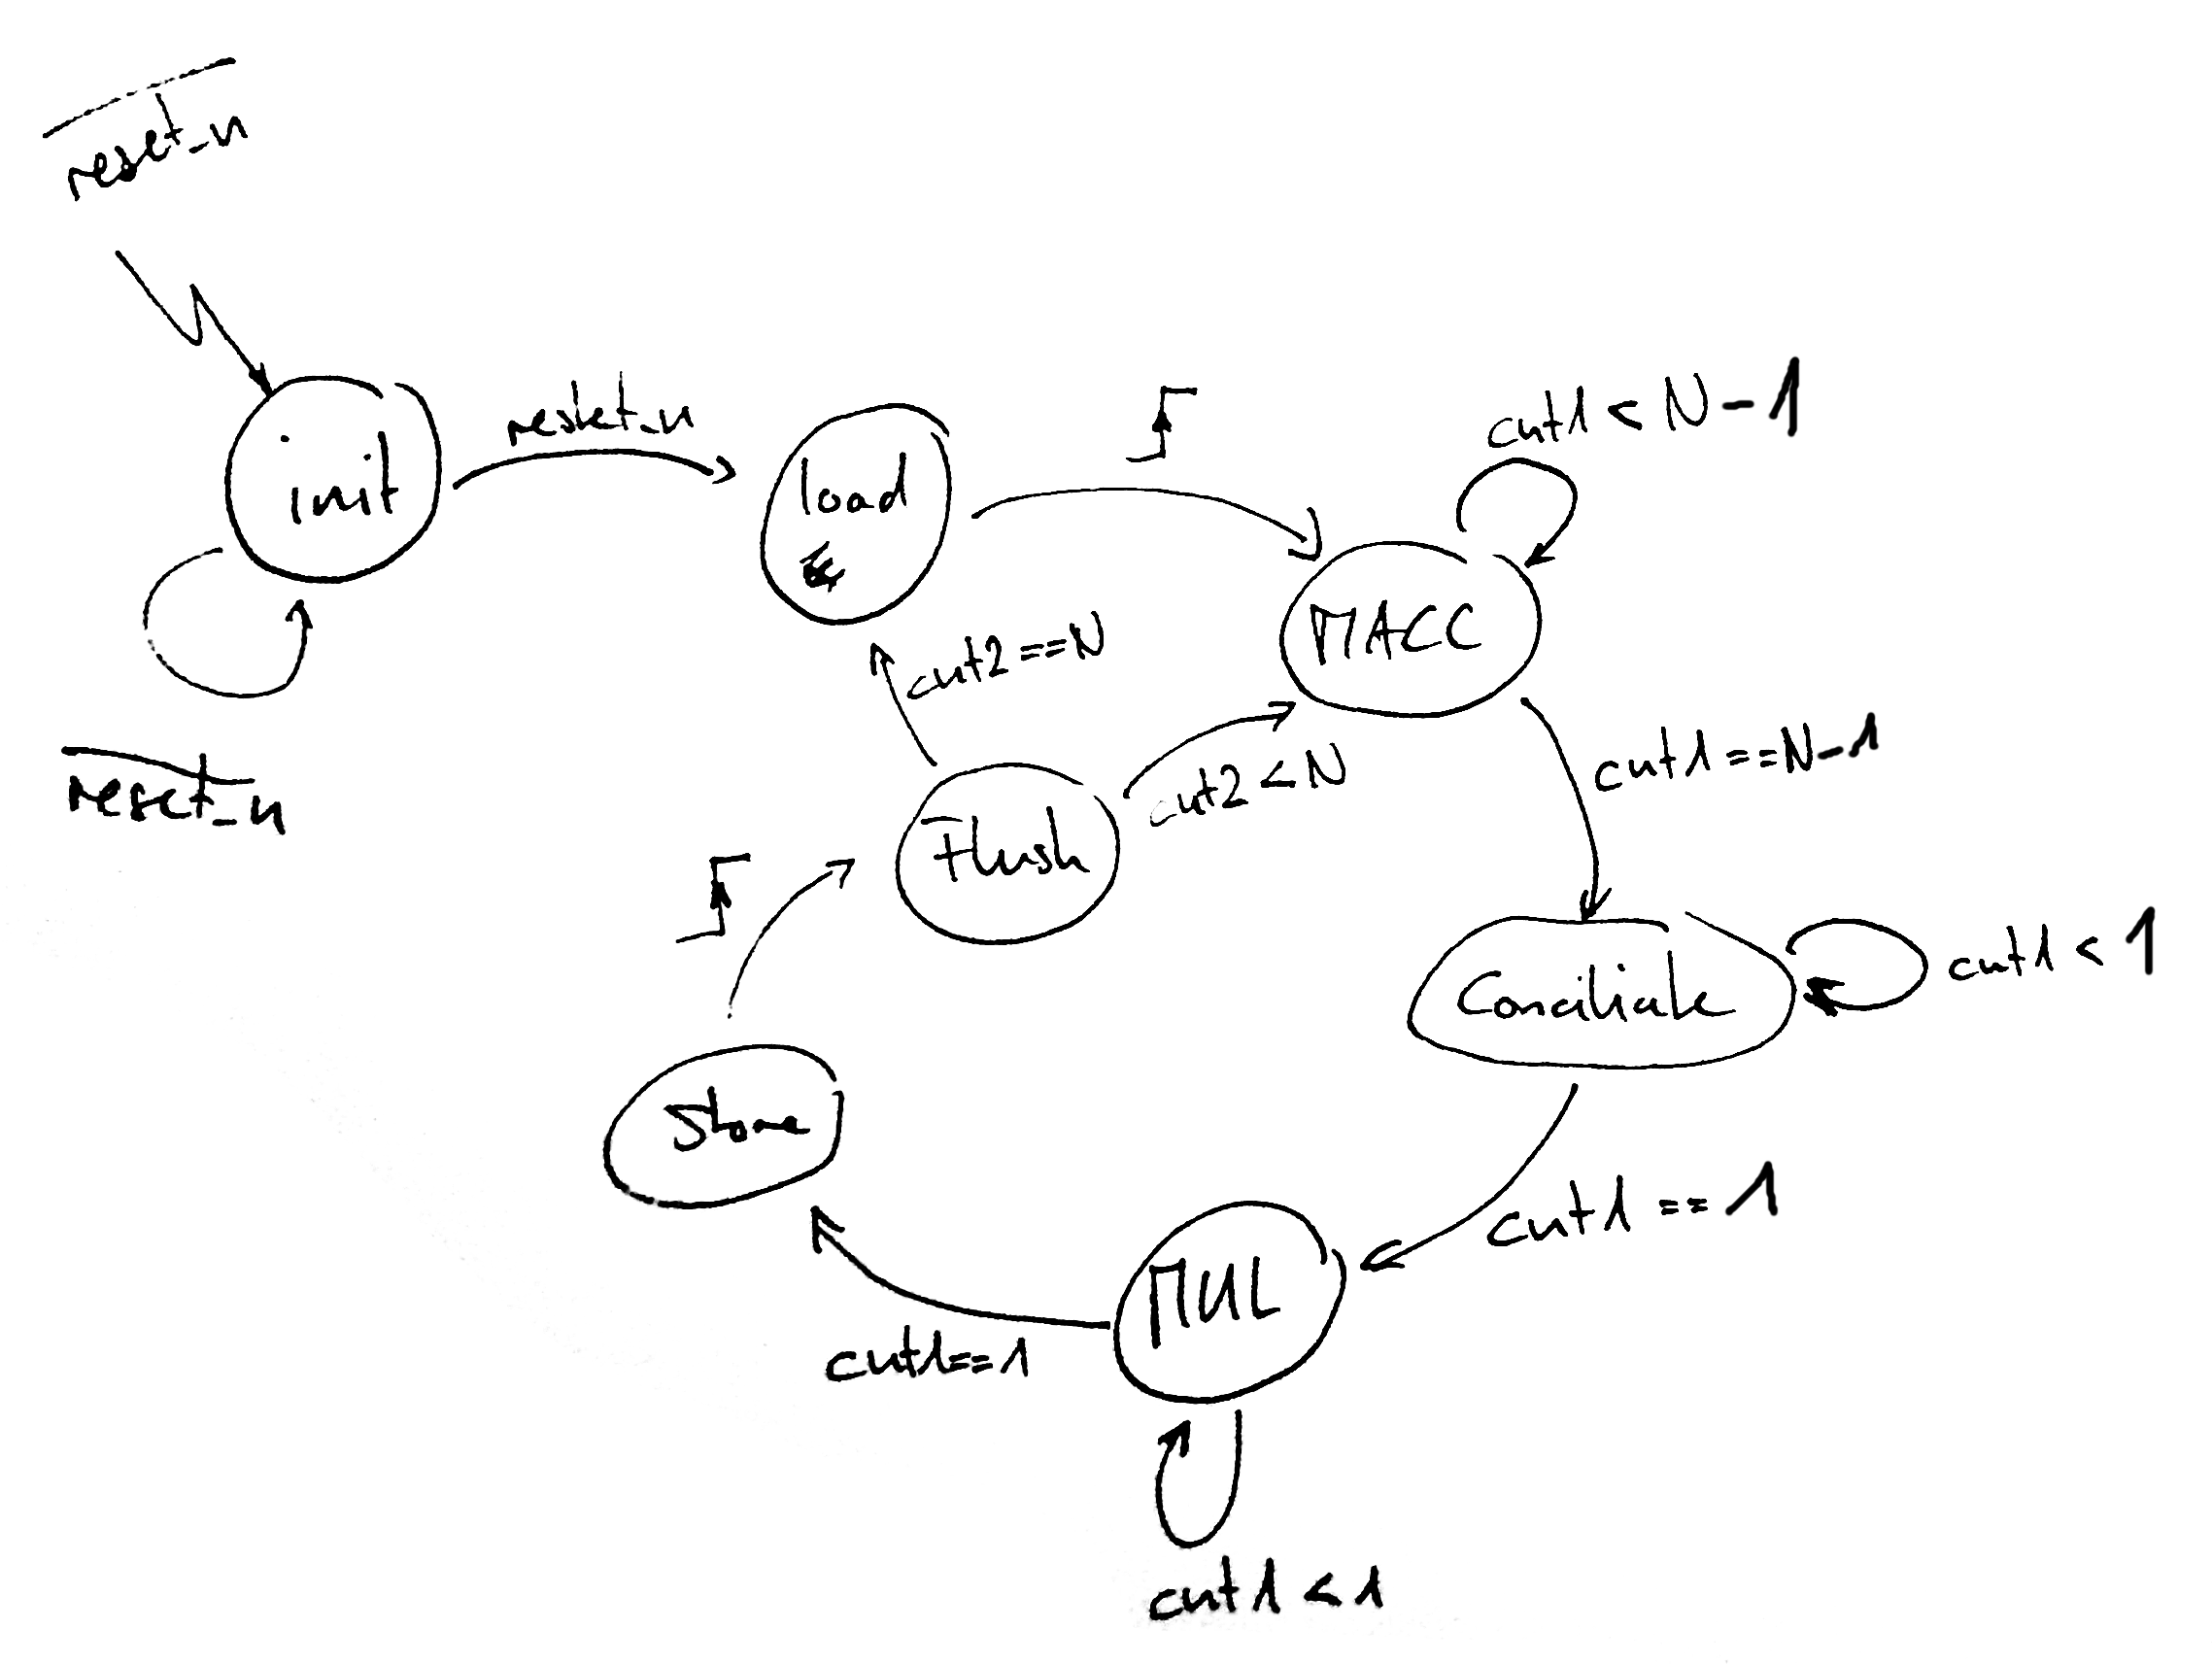
\includegraphics[width=1\columnwidth]{./schema/arch_ctrl.png}
    \caption{controller of serial implementation}
    \label{fig:ctrl}
\end{figure}

\emph{\color{red} in table \ref{tab:ctrl} the signals flush\_ps and load\_out
are only set in the first iteration. add a footnote?}

%\begin{table}
%    \begin{center}
%    \begin{tabular}{|l|c|c|c|c|c|c|c|}
%    \hline
%    signal            & init & select & macc & conciliate & mul & store & flush \\
%    \hline
%    \hline
%    shift\_alpha\_in  & 0    & 0      & 1    & 0          & 0   & 0     & 0     \\
%    shift\_alpha\_out & 0    & 0      & 0    & 0          & 0   & 1     & 0     \\
%    conciliate        & 0    & 0      & 0    & 1          & 0   & 0     & 0     \\
%    enable\_init      & 0    & 0      & 0    & 0          & 1   & 0     & 0     \\
%    enable\_step      & 0    & 0      & 1    & 1          & 1   & 0     & 0     \\
%    enable\_final     & 0    & 1      & 0    & 0          & 0   & 0     & 0     \\
%    flush             & 0    & 0      & 0    & 0          & 0   & 0     & 1     \\
%    \hline
%    \end{tabular}
%    \end{center}
%    \caption{control signals}
%    \label{tab:ctrl}
%\end{table}

\begin{table}
    \footnotesize
    \begin{center}
    \begin{tabular}{|c|l|*{10}{c|}}
    \hline
    type & signal                      & init & select & macc & conciliate & shift1 & shift2 & mul & store & flush & input       \\
    \hline
    \hline
         & pi\_we                      &      &        &      &            &        &        &      &      &       & input       \\
         & tp\_we                      &      &        &      &            &        &        &      &      &       & input       \\
         & b\_we                       &      &        &      &            &        &        &      &      &       & input       \\
         & data\_ready                 &      &        &      &            &        &        &      &      &       & input       \\
    1    & enable\_count               & 0    & 0      & 0    & 0          & 0      & 0      & 0    & 1    & 0     & pi\_we      \\
    2    & enable\_ctrl                & 0    & 0      & 0    & 0          & 0      & 0      & 0    & 0    & 0     & data\_ready \\
    3    & enable\_init                & 0    & 0      & 0    & 0          & 0      & 0      & 1    & 0    & 0     & data\_ready \\
    3    & enable\_init\_mul           & 0    & 0      & 0    & 0          & 0      & 0      & 1    & 0    & 0     & data\_ready \\
    4    & enable\_step                & 0    & 0      & 1    & 1          & 1      & 1      & 1    & 0    & 0     & data\_ready \\
    4    & enable\_step\_macc          & 0    & 0      & 1    & 1          & 1      & 1      & 1    & 0    & 0     & data\_ready \\
    5    & enable\_final               & 0    & 1      & 0    & 0          & 0      & 0      & 0    & 0    & 0     & data\_ready \\
    4    & laod\_op2                   & 0    & 0      & 1    & 1          & 1      & 1      & 1    & 0    & 0     & data\_ready \\
    6    & load\_step\_alpha           & 0    & 0      & 1    & 0          & 0      & 0      & 0    & 0    & 0     &             \\
    7    & load\_final\_alpha          & 0    & 0      & 0    & 0          & 0      & 0      & 0    & 1    & 0     &             \\
    8    & load\_scale\_new            & 0    & 1(d)   & 0    & 0          & 0      & 0      & 0    & 0    & 0     &             \\
    9    & load\_scale\_acc            & 0    & 1      & 0    & 0          & o      & 0      & 0    & 0    & 0     &             \\
    7    & store\_init\_scale\_new     & 0    & 0      & 0    & 0          & 0      & 0      & 0    & 1    & 0     &             \\
    23   & store\_init\_scale\_small   &      & 1(d)   &      &            &        &        &      &      &       & or internal \\
    9    & store\_init\_scale\_ok      & 0    & 1      & 0    & 0          & 0      & 0      & 0    & 0    & 0     &             \\
    7    & store\_step\_alpha          & 0    & 0      & 0    & 0          & 0      & 0      & 0    & 1    & 0     &             \\
    7    & store\_step\_scale\_new     & 0    & 0      & 0    & 0          & 0      & 0      & 0    & 1    & 0     &             \\
    23   & store\_step\_scale\_small   &      & 1(d)   &      &            &        &        &      &      &       & or internal \\
    9    & store\_step\_scale\_ok      & 0    & 1      & 0    & 0          & 0      & 0      & 0    & 0    & 0     &             \\
    5    & store\_final\_ps            & 0    & 1      & 0    & 0          & 0      & 0      & 0    & 0    & 0     & data\_ready \\
    10   & store\_final\_ps\_delayed   & 0    & 1(d)   & 0    & 0          & 0      & 0      & 0    & 0    & 0     & data\_ready \\
    10   & store\_final\_scale         & 0    & 1(d)   & 0    & 0          & 0      & 0      & 0    & 0    & 0     & data\_ready \\
    11   & shift\_step\_acc            & 0    & 0      & 0    & 1(6)       & 0      & 0      & 0    & 0    & 0     &             \\
    12   & sel\_mux2\_op2              & 0    & 0      & 0    & 0          & 0      & 0      & 1    & 0    & 0     &             \\
    13   & sel\_step\_read\_fifo       &      & (*)    &      &            &        &        &      &      &       & special     \\
    12   & sel\_step\_op1              & 0    & 0      & 0    & 0          & 0      & 0      & 1    & 0    & 0     &             \\
    14   &                             & 0    & 0      & 0    & 1          & 1      & 0      & 0    & 0    & 0     &             \\
    15   &                             & 0    & 0      & 0    & 1          & 0      & 1      & 0    & 0    & 0     &             \\
    16   & sel\_step\_op2              & 0    & 0      & 0    & 1(5)       & 1      & 1      & 0    & 0    & 0     &             \\
    17   & flush\_init                 & 0    & 0      & 0    & 0          & 0      & 0      & 0    & 0    & 1     &             \\
    17   & flush\_step\_macc           & 0    & 0      & 0    & 0          & 0      & 0      & 0    & 0    & 1     &             \\
    18   & flush\_step\_acc            & 0    & 0      & 0    & 0          & 0      & 1      & 0    & 0    & 0     &             \\
    9    & flush\_step\_fifo           & 0    & 1      & 0    & 0          & 0      & 0      & 0    & 0    & 0     &             \\
         & reset\_n                    & 0    & 0      & 0    & 0          & 0      & 0      & 0    & 0    & 0     & input       \\
    19   & reset\_count\_n             & 0    & 0      & 0    & 0          & 0      & 0      & 0    & 0    & 0     & reset\_n    \\
    19   & reset\_op2\_n               & 0    & 0      & 0    & 0          & 0      & 0      & 0    & 0    & 0     & reset\_n    \\
    19   & reset\_ctrl\_n              & 0    & 0      & 0    & 0          & 0      & 0      & 0    & 0    & 0     & reset\_n    \\
    19   & reset\_init\_n              & 0    & 0      & 0    & 0          & 0      & 0      & 0    & 0    & 0     & reset\_n    \\
    20   & reset\_init\_mul\_n         & 0    & 0      & 0    & 0          & 0      & 0      & 0    & 0    & 1(n)  & reset\_n    \\
    19   & reset\_step\_n              & 0    & 0      & 0    & 0          & 0      & 0      & 0    & 0    & 0     & reset\_n    \\
    20   & reset\_step\_macc\_n        & 0    & 0      & 0    & 0          & 0      & 0      & 0    & 0    & 1(n)  & reset\_n    \\
    21   & reset\_step\_fifo0          & 0    & 1(*(n))& 0    & 0          & 0      & 0      & 0    & 0    & 0     & reset       \\
    22   & reset\_step\_fifo1          & 0    & 1(*)   & 0    & 0          & 0      & 0      & 0    & 0    & 0     & reset       \\
    19   & reset\_step\_scale\_new\_n  & 0    & 0      & 0    & 0          & 0      & 0      & 0    & 0    & 0     & reset\_n    \\
    19   & reset\_step\_scale\_small\_n& 0    & 0      & 0    & 0          & 0      & 0      & 0    & 0    & 0     & reset\_n    \\
    19   & reset\_step\_scale\_ok\_n   & 0    & 0      & 0    & 0          & 0      & 0      & 0    & 0    & 0     & reset\_n    \\
    19   & reset\_init\_scale\_new\_n  & 0    & 0      & 0    & 0          & 0      & 0      & 0    & 0    & 0     & reset\_n    \\
    19   & reset\_init\_scale\_small\_n& 0    & 0      & 0    & 0          & 0      & 0      & 0    & 0    & 0     & reset\_n    \\
    19   & reset\_init\_scale\_ok\_n   & 0    & 0      & 0    & 0          & 0      & 0      & 0    & 0    & 0     & reset\_n    \\
    19   & reset\_final\_n             & 0    & 0      & 0    & 0          & 0      & 0      & 0    & 0    & 0     & reset\_n    \\
    \hline
    \end{tabular}
    \end{center}
    \caption{detailed control signals}
    \label{tab:ctrl_detailed}
\end{table}

%-------------------------------------------------------------------------------
%===============================================================================
\section{balancing pipeline stages}

%-------------------------------------------------------------------------------
%===============================================================================
\section{practical notes}

\begin{itemize}
    \item generic design (change n, l and bit widths in param\_pkg)
    \item if bit widths of op1 is changed, fifo\_512x25 must be regenerated
\end{itemize}

%===============================================================================
%%%%%%%%%%%%%%%%%%%%%%%%%%%%%%%%%%%%%%%%%%%%%%%%%%%%%%%%%%%%%%%%%%%%%%%%%%%%%%%%
\chapter{testing and verification}
\label{ch:test}

%-------------------------------------------------------------------------------
%===============================================================================
\section{device}
\label{ch:test_dev}

\begin{itemize}
    \item nexys4 board with artix-7 fpga
    \item limited recourses -> proof of concept
    \item bord hardware for testing
\end{itemize}

%-------------------------------------------------------------------------------
%===============================================================================
\section{relation to proposed algorithm}
\label{ch:test_prop}

%-------------------------------------------------------------------------------
\subsection{log standard}

%-------------------------------------------------------------------------------
\subsection{metrics}

%===============================================================================
%%%%%%%%%%%%%%%%%%%%%%%%%%%%%%%%%%%%%%%%%%%%%%%%%%%%%%%%%%%%%%%%%%%%%%%%%%%%%%%%
\chapter{results}
\label{ch:res}
%-------------------------------------------------------------------------------
\section{speedup}
\label{ch:res_speed}
%-------------------------------------------------------------------------------
\section{accuracy}
\label{ch:res_prec}

%===============================================================================
%%%%%%%%%%%%%%%%%%%%%%%%%%%%%%%%%%%%%%%%%%%%%%%%%%%%%%%%%%%%%%%%%%%%%%%%%%%%%%%%
\chapter{conclusion}
\label{ch:conc}

%-------------------------------------------------------------------------------
%===============================================================================
\section{achievements}
\label{ch:conc_ach}

%-------------------------------------------------------------------------------
%===============================================================================
\section{future work}
\label{ch:conc_work}

\nocite{*}

\appendix %optional, use only if you have an appendix

%===============================================================================
%%%%%%%%%%%%%%%%%%%%%%%%%%%%%%%%%%%%%%%%%%%%%%%%%%%%%%%%%%%%%%%%%%%%%%%%%%%%%%%%
\chapter{some material}
%\section{it's over\dots}

\backmatter

%\chapter{glossary} %optional

%\bibliographystyle{alpha}
%\bibliographystyle{dcu}
%\bibliographystyle{plainnat}
%\bibliographystyle{plain}
%\bibliographystyle{abbrvnat}
\bibliographystyle{siam}
%\bibliographystyle{ieeetr}
\bibliography{biblio}

%\cleardoublepage
%\theindex %optional, use only if you have an index, must use
	  %\makeindex in the preamble

\end{document}
